%% Преамбула TeX-файла

% 1. Стиль и язык
\documentclass[utf8x, 12pt]{G7-32} % Стиль (по умолчанию будет 14pt)

% Остальные стандартные настройки убраны в preamble.inc.tex.
\sloppy

% Настройки стиля ГОСТ 7-32
% Для начала определяем, хотим мы или нет, чтобы рисунки и таблицы нумеровались в пределах раздела, или нам нужна сквозная нумерация.
\EqInChapter % формулы будут нумероваться в пределах раздела
\TableInChapter % таблицы будут нумероваться в пределах раздела
\PicInChapter % рисунки будут нумероваться в пределах раздела

% Добавляем гипертекстовое оглавление в PDF
\usepackage[
bookmarks=true, colorlinks=true, unicode=true,
urlcolor=black,linkcolor=black, anchorcolor=black,
citecolor=black, menucolor=black, filecolor=black,
]{hyperref}

% Изменение начертания шрифта --- после чего выглядит таймсоподобно.
% apt-get install scalable-cyrfonts-tex

\IfFileExists{cyrtimes.sty}
    {
        \usepackage{cyrtimespatched}
    }
    {
        % А если Times нету, то будет CM...
    }

\usepackage{graphicx}   % Пакет для включения рисунков

% С такими оно полями оно работает по-умолчанию:
% \RequirePackage[left=20mm,right=10mm,top=20mm,bottom=20mm,headsep=0pt]{geometry}
% Если вас тошнит от поля в 10мм --- увеличивайте до 20-ти, ну и про переплёт не забывайте:
\geometry{right=20mm}
\geometry{left=30mm}


% Пакет Tikz
\usepackage{tikz}
\usetikzlibrary{arrows,positioning,shadows}

% Произвольная нумерация списков.
\usepackage{enumerate}


% Настройки листингов.
% 8 Листинги

\usepackage{listings}

% Значения по умолчанию
\lstset{
  basicstyle= \footnotesize,
  breakatwhitespace=true,% разрыв строк только на whitespacce
  breaklines=true,       % переносить длинные строки
%   captionpos=b,          % подписи снизу -- вроде не надо
  inputencoding=koi8-r,
  numbers=left,          % нумерация слева
  numberstyle=\footnotesize,
  showspaces=false,      % показывать пробелы подчеркиваниями -- идиотизм 70-х годов
  showstringspaces=false,
  showtabs=false,        % и табы тоже
  stepnumber=1,
  tabsize=4,              % кому нужны табы по 8 символов?
  frame=single
}

% Стиль для псевдокода: строчки обычно короткие, поэтому размер шрифта побольше
\lstdefinestyle{pseudocode}{
  basicstyle=\small,
  keywordstyle=\color{black}\bfseries\underbar,
  language=Pseudocode,
  numberstyle=\footnotesize,
  commentstyle=\footnotesize\it
}

% Стиль для обычного кода: маленький шрифт
\lstdefinestyle{realcode}{
  basicstyle=\scriptsize,
  numberstyle=\footnotesize
}

% Стиль для коротких кусков обычного кода: средний шрифт
\lstdefinestyle{simplecode}{
  basicstyle=\footnotesize,
  numberstyle=\footnotesize
}

% Стиль для BNF
\lstdefinestyle{grammar}{
  basicstyle=\footnotesize,
  numberstyle=\footnotesize,
  stringstyle=\bfseries\ttfamily,
  language=BNF
}

% Определим свой язык для написания псевдокодов на основе Python
\lstdefinelanguage[]{Pseudocode}[]{Python}{
  morekeywords={each,empty,wait,do},% ключевые слова добавлять сюда
  morecomment=[s]{\{}{\}},% комменты {а-ля Pascal} смотрятся нагляднее
  literate=% а сюда добавлять операторы, которые хотите отображать как мат. символы
    {->}{\ensuremath{$\rightarrow$}~}2%
    {<-}{\ensuremath{$\leftarrow$}~}2%
    {:=}{\ensuremath{$\leftarrow$}~}2%
    {<--}{\ensuremath{$\Longleftarrow$}~}2%
}[keywords,comments]

% Свой язык для задания грамматик в BNF
\lstdefinelanguage[]{BNF}[]{}{
  morekeywords={},
  morecomment=[s]{@}{@},
  morestring=[b]",%
  literate=%
    {->}{\ensuremath{$\rightarrow$}~}2%
    {*}{\ensuremath{$^*$}~}2%
    {+}{\ensuremath{$^+$}~}2%
    {|}{\ensuremath{$|$}~}2%
}[keywords,comments,strings]

% Подписи к листингам на русском языке.
\renewcommand\lstlistingname{\cyr\CYRL\cyri\cyrs\cyrt\cyri\cyrn\cyrg}
\renewcommand\lstlistlistingname{\cyr\CYRL\cyri\cyrs\cyrt\cyri\cyrn\cyrg\cyri}


% Полезные макросы листингов.
% Любимые команды
\newcommand{\Code}[1]{\textbf{#1}}


\begin{document}

\frontmatter % выключает нумерацию ВСЕГО; здесь начинаются ненумерованные главы: реферат, введение, глоссарий, сокращения и прочее.

% Команды \breakingbeforechapters и \nonbreakingbeforechapters
% управляют разрывом страницы перед главами.
% По-умолчанию страница разрывается.

% \nobreakingbeforechapters
% \breakingbeforechapters

% Также можно использовать \Referat, как в оригинале
\begin{abstract}
В данной работе представлено описание разработки метода сжатия видео.

Цель работы: разработка метода сжатия видео на основе кратномасштабного анализа.

В дипломной работе приводится анализ существующих алгоритмов сжатия видео. Выделяются особенности существующих
алгоритмов, их достоинства и недостатки. Приводится сравнение существующих алгоритмов сжатия видео.

Был предложен метод сжатия видео на основе кратномасштабного анализа, разработан алгоритм на основе 
предложенного метода. Также был создан программный комплекс, позволяющий применять разработанный алгоритм к видео.

В работе было проведено исследование исследование работы предложенного метода. Были определены типы видео,
применение метода к которым дает наиболее эффективное сжатие видео.


\end{abstract}

%%% Local Variables: 
%%% mode: latex
%%% TeX-master: "rpz"
%%% End: 


\tableofcontents

\Defines % Необходимые определения. Вряд ли понадобться
\begin{description}
\item[Вейвлетное преобразование (англ. wavelet transform)] Инструмент, разбивающий данные, или функции, 
или операторы на составляющие с разными частотами, каждая из которых затем изучается с разрешением, подходящим по масштабу \cite{Pup01}
\end{description}
\begin{description}
\item[Битрейт] Величина потока данных, передаваемого в реальном времени (минимальный размер канала, который сможет пропустить этот поток без задержек). Частный случай — битрейт сжатого звука или видео.
\end{description}
\begin{description}
\item[Класс изображений/видео] совокупность изображений/видео, применение к которым алгоритма архивации дает качественно одинаковые результаты \cite{Pup02}
\end{description}
\begin{description}
\item[Коэффициент сжатия] отношение длины сжатых данных к длине соответствующих им несжатых данных \cite{Pup02}
\end{description}
\begin{description}
\item[Степень сжатия] отношение длины несжатых данных к длине соответствующих им сжатых данных \cite{Pup02}
\end{description}
\begin{description}
\item[Порядковая статистика (order statistic)] i-я порядковая статистика множества, состоящего из n элементов – это i-й элемент в порядке возрастания \cite{Pup05}
\end{description}
\begin{description}
\item[Цифровое видео] последовательность кадров, в которой каждый кадр рассматривается как набор отсчетов аналогового изображения. Отсчеты - пиксели \cite{Pup07}
\end{description}
%%% Local Variables:
%%% mode: latex
%%% TeX-master: "rpz"
%%% End:

\Abbreviations %% Список обозначений и сокращений в тексте
\begin{description}
\item[АИС] Автоматизированная информационная система. Но надо протестировать длинные строки в определениях.
\end{description}

%%% Local Variables:
%%% mode: latex
%%% TeX-master: "rpz"
%%% End:


\Introduction

Развитие интернета, рост производительности компьютеров и прогресс в технологии 
производства цифровых камер, сканеров и принтеров привели к широкому использованию 
цифровых данных, в том числе видео. В последнее время наблюдается бурное развитие 
телекоммуникационных систем, предназначенных для приема и передачи 
видеоданных. 
Для хранения видео информации требуется 
больший объем, чем для других типов данных, таких как звуковая, текстовая информация или изображения. 
С ростом разрешающей способности экранов современных персональных компьютеров, а так же экранов кинотеатров
качество видео и их размер постоянно растут. 
Размер графических данных файла с видео пропорционален количеству кадров, количеству пикселей в 
каждом кадре и количеству битов, требуемых для представления глубины цвета каждого пикселя. 
Без использования алгоритмов сжатия файл с графическими данными может занимать объем, сопоставимый с 
емкостью носителей современных персональных компьютеров. 
Необходимо улучшать алгоритмы сжатия данных, представляющих цифровой поток видеоданных. 
Сжатие данных важно как для скорости передачи, так и для эффективности хранения \cite{Pup03}.

В настоящее время разработаны алгоритмы сжатия без потерь на основе универсальных 
методов сжатия и алгоритмы сжатия с потерями, использующие особенности графических 
данных. Продолжаются работы над алгоритмами сжатия с потерями, сохраняющими качество 
видео на высоком уровне.

Области применения методов кодирования и сжатия видеоинформации весьма разнообразны:
от передачи и хранения видео до спутниковых цифровых телекоммуникационных систем. 
Внимание к сжатию видеоинформации особенно возросло в последнее десятилетие в связи с 
разработкой принципиально новых цифровых телекоммуникационных систем. Создание новейших
цифровых устройств обработки, передачи и хранения видеоизображений связано с радикальным
изменением технологических возможностей новейших процессорных систем, создаваемых ведущими
мировыми фирмами, специализирующимися в области совершенствования аппаратных и программных 
компьютерных средств. Использование новейших процессоров с производительностью несколько 
миллиардов операций в секунду обеспечивает реализацию самых сложных и вычислительно емких 
алгоритмов сжатия, что невозможно было осуществить ранее \cite{Pup07}. 

Передача цифрового видео от источника (видеокамера или записанный 
видеоролик) к получателю (видеодисплей) вовлекает в разработку целую цепь 
различных компонентов и процессов. Ключевыми звеньями этой цепи являются 
процесс компрессии (кодирования) и декомпрессии (декодирования), при 
которых несжатый цифровой видеосигнал сокращается до размеров, 
подходящих для его передачи и хранения, а затем восстанавливается для 
отображения на видеоэкране. 
Продуманная разработка процессов компрессии и декомпрессии может 
дать существенное коммерческое и техническое преимущество продукта, 
обеспечив лучшее качество видеоизображения, большую надежность и гибкую 
приспособляемость по сравнению с конкурирующими решениями. 
Таким образом, имеется заинтересованность в развитии и 
улучшении методов компрессии и декомпрессии видео \cite{Pup13}.

\mainmatter % это включает нумерацию глав и секций в документе ниже

\chapter{Аналитический раздел}
\label{cha:analysis}

\section{Цель разработки и основные решаемые задачи}

Цель настоящей работы – разработать метод сжатия видео на основе кратномасштабного анализа. 
Задачи настоящей работы:        

\begin{itemize}
\item провести анализ существующих методов сжатия видео,
\item разработать метод сжатия видео на основе кратномасштабного анализа,
\item создать приложение, позволяющее применять разработанный метод к видео,
\item разработать модель для оценки предложенного метода,
\item провести исследование работы метода.
\end{itemize}

\section{Анализ алгоритмов сжатия видео}

\subsection{Характеристики видео}

Видео (от лат. video — смотрю, вижу) — электронная технология формирования, записи, 
обработки, передачи, хранения и воспроизведения сигналов изображения.

Цифровое видео — множество технологий записи, обработки, передачи, 
хранения и воспроизведения визуального или аудиовизуального материала в цифровом представлении. Основное 
отличие от аналогового видео в том, что видеосигналы кодируются и передаются 
в виде последовательности бит. Цифровое видео может распространяться на 
различных видеоносителях, посредством цифровых видеоинтерфейсов в виде потока или файлов.

Этот тип данных имеет следующие характеристики:
\begin{itemize}
\item Разрешающая способность.
Любой цифровой видеосигнал характеризуется разрешением (англ. resolution), 
горизонтальным и вертикальным, измеряемым в пикселях. Разрешение обозначается двумя числами, где
первым числом обозначается количество точек в строке (горизонтальное разрешение), 
а вторым числом количество активных строк, участвующих в построении изображения 
(вертикальное разрешение). 

\item Количество цветов и цветовое разрешение.
Количество цветов и цветовое разрешение видеозаписи описывается цветовыми моделями. 
Для различных стандартов применяются различные цветовые модели: YUV, YDbDr, YIQ, RGB (и ARGB), HSV, CMYK. 
Человеческий глаз может воспринять, по разным подсчётам, от 5 до 10 миллионов оттенков цветов. 
Количество цветов в видеозаписи определяется числом бит, отведённым для кодирования цвета каждого 
пикселя (англ. bits per pixel, bpp). 

\item Битрейт (ширина видеопотока или информационная скорость записи).
Ширина видеопотока или битрейт (англ. bit rate) — это количество обрабатываемых бит 
видеоинформации за секунду времени (измеряется «бит/с» — бит в секунду или, чаще, «Мб/с» — 
мегабит в секунду; в английском обозначении bit/s и Mbit/s соответственно). 
Чем выше ширина видеопотока, тем, как правило, лучше качество видео. 
Различают два вида управления шириной потока в видеокодеке — постоянный битрейт 
(англ. constant bit rate, CBR) и переменный битрейт (англ. variable bit rate, VBR). 
Концепция VBR разработана для максимального сохранения качества видео, 
уменьшая при этом суммарный объём передаваемого видеопотока. 
При этом на быстрых сценах движения, ширина видеопотока возрастает, 
а на медленных сценах, где картинка меняется медленно, ширина потока падает. 
Это удобно для буферизованных видеотрансляций и передачи сохранённого видеоматериала 
по компьютерным сетям. Но для безбуферных систем реального времени и для прямого эфира 
(например, для телеконференций) это не подходит — в этих случаях необходимо 
использовать постоянную скорость видеопотока.

\item Качество видео.
Качество видеозаписи измеряется с помощью формальных метрик, таких как PSNR или SSIM, 
или с использованием субъективного сравнения с привлечением экспертов.

Качество видео может быть оценено субъективно по следующей методике:

\begin{enumerate}
\item выбираются видеопоследовательности для использования в тесте
\item выбираются параметры системы измерения
\item выбирается метод показа видео и подсчета результатов измерения
\item приглашается необходимое число экспертов (обычно не меньше 15)
\item проводится сам тест
\item подсчитывается средняя оценка на основе оценок экспертов.
\end{enumerate}

\end{itemize}

\subsection{Сжатие видео}

Сжатие видео (англ. Video compression) — технология компрессии цифрового видео, 
позволяющая сократить количество данных, используемых для представления видеопотока. 
Сжатие видео позволяет эффективно уменьшать поток, необходимый для передачи 
видео по каналам связи, уменьшать пространство, необходимое для хранения данных на носителе. 

Скорости передачи данных в сетях, а также емкости жестких дисков,
флэш-памяти и оптических накопителей постоянно растут. Не смотря на
снижение цены передачи и хранения бита информации, видеосжатие и его улучшение является необходимым.
Видеосжатие имеет важные преимущества. Во-первых, оно дает возможность
использовать цифровое видео в среде передачи и хранения видеоконтента,
которая не поддерживает несжатое видео. Например, пропускная
способность современного Интернета недостаточна для обращения с несжатым
видео в реальном масштабе времени даже при низкой частоте кадра и малом его
размере. Цифровой многослойный видеодиск DVD может вместить всего
несколько секунд несжатого видео с разрешением и частотой кадров,
обеспечивающими обычное телевизионное качество, поэтому использование
DVD было бы абсолютно непрактичным без применения аудио и видеосжатия.
Во-вторых, видеосжатие делает более эффективным использование ресурсов
при передаче и хранении видеоданных. Если доступен высокоскоростной
канал, то более привлекательным представляется решение, позволяющее
передавать сжатое видео высокого разрешения вместо несжатого видео
низкого разрешения. Несмотря на постоянный рост емкости устройств
хранения информации и пропускной способности каналов передачи данных,
представляется весьма вероятным, что сжатие видео остается
существенным компонентом мультимедийных сервисов.

Сигнал, несущий определенную информацию, можно сжать путем
удаления из него имеющейся избыточности. Избыточность – это компоненты
данных, без которых можно обойтись для верного отображения исходной 
информации. Многие типы данных содержат в себе статистическую
избыточность. Такие данные могут быть эффективно сжаты с использованием
алгоритмов сжатия без потерь. Сжатие без потерь применительно к
видео не является эффективным. Поэтому для достижения
высокой эффективности сжатия применяется сжатие с потерями. При
сжатии видео с потерями используется несколько типов избыточности:
\begin{itemize}
\item когерентность областей изображения - малое изменение цвета изображения
в соседних пикселях (свойство, которое используется в алгоритмах
сжатия изображений с потерями),
\item избыточность в цветовых плоскостях - используется важность
яркости изображения для восприятия,
\item подобие между кадрами - использование того факта, что на скорости 25
кадров в секунду, как правило, соседние кадры изменяются незначительно.
\end{itemize}

Использование подобия между кадрами в самом простом и наиболее
часто используемом случае означает кодирование не самого нового кадра, а его
разности с предыдущим кадром. Для видео, на котором нет большого количетсва движения (передача
новостей, видеотелефоны, съемка с камер наблюдения) большая часть кадра остается неизменной, и
такой метод позволяет значительно уменьшить поток данных. Более
сложный метод заключается в нахождении для каждого блока в сжимаемом
кадре наименее отличающегося от него блока в кадре, используемом в качестве
базового. Далее кодируется разница между этими блоками. Этот метод
существенно более ресурсоемкий.

При сравнении алгоритмов сжатия видео необходимо учитывать следующие особенности видео:

\begin{itemize}
\item Качество различных кадров одного и того же видео после обработки одним алгоритмом отличается.
Это связано с несколькими факторами. Качество может меняться в зависимости от стратегии управления битрейтом. 
Пользователь выбирает разные стратегии битрейта, и в случае выбора постоянного битрейта
на медленных сценах качество будет высоким, а на быстрых - низким. У кодеков есть так называемые 
ключевые кадры, качество которых обычно изменяется отдельно, и отличается от качества остальных кадров. 
На качество влияет префильтрация. Это означает, что на любом достаточно длинном видео можно подобрать 
как достаточно хорошие, так и достаточно плохие кадры. 

\item Алгоритмы сжатия видео создаются для различных типов видео.
Один и тот же алгоритм при различных параметрах, но одинаковом формате сжатия может по-разному сжимать различные видео, отличающиеся, например, наличием большого 
количества движения. Это означает, что для двух различных алгоритмов примерно равного качества можно подобрать видео, на которых первый будет заметно лучше второго и наоборот.

\item Качество сжатия видео зависит от параметров кодирования. 
У алгоритмов есть достаточно много параметров, позволяющих при том же размере файла заметно изменить качество. Это параметры стратегии битрейта, префильтрации, управления частотой ключевых кадров, управление зависимости префильтра от видео и другие. Это означает, что для одного и того же видео и при использовании одного алгоритма при указании различных параметров размер файла может быть одинаковым, но сильно отличаться по качеству.

\end{itemize}

В настоящее время существуют следующие алгоритмы сжатия видео:
\begin{itemize}
\item сжатие без потерь

При декомпрессии результат в точности соответствует оригиналу. При сжатии без потерь 
невозможно получить высокие коэффициены сжатия. По этой причине практически всё
широко используемое видео является сжатым с потерями. Краткое сравнение алгоритмов сжатия видео без потерь представлено в таблице \ref{tab:t1}.

\begin{enumerate}
\item HuffYUV

Каждый кадр сжимается отдельно при помощи алгоритма Хаффмана. 
Если часть кадра постоянно занимает однородный фон, то потребуется меньший поток данных, 
например для записей широкоэкранных кинофильмов (с чёрными полосами сверху и снизу изображения). 

\item CorePNG

Каждый кадр видео сжимается с использованием алгоритма сжатия PNG, позволяя 
использовать все возможности PNG формата, но также наследуя все его недостатки.
CorePNG поддерживает кодирование видео в цветовом пространстве RGB с глубиной 
цвета 24 или 32 бит. 32-битная глубина позволяет использовать необязательный 
альфа-канал. Поддержка других цветовых пространств, таких как YUY2 или YV12, также предоставляется.
CorePNG поддерживает запись P-кадров, называемых delta кадрами, в видеопотоке они 
кодируют только различия между предыдущим и текущим кадрами. 

\item Lagarith

Базируется на Huffyuv, примерно сравним с ним по быстродействию, превосходит по степени сжатия. 
Хорошо сжимает видео с преобладанием статических изображений. Это достигается 
за счёт поддержки недействительных фреймов, то есть если предшествующий фрейм 
идентичен текущему, то он используется снова, а текущий отвергается.
Lagarith работает в цветовых пространствах RGB24, RGB32, RGBA, YUY2 и YV12.
Последние версии поддерживают многопроцессорность. 
Каждый кадр может быть отдельно декодирован, это облегчает поиск, вырезание, объединение.

\item Motion JPEG 2000 

Это система кодирования видеоизображения с применением внутрикадровой технологии сжатия JPEG 2000, 
разработанная институтом интегральных схем общества Фраунгофера. 
В основе лежит дискретное вейвлет-преобразование, которое, в отличие от 
дискретно-косинусного преобразования, применяемого в кодеках семейства MPEG, 
производит кодирование сразу в двух областях: и в частотной, и в пространственной. 
Это исключает необходимость разбиения изображения на блоки. Для каждого кадра 
применяется только внутрикадровое сжатие без использования межкадрового кодирования.
Отличительной особенностью является возможность масштабируемости, 
причем не только по размеру кадра, но и по качеству, 
то есть скорости видеопотока. Из-за особенностей вейвлет разложения, каждый 
кадр может содержать свои копии, уменьшенные вдвое по горизонтали и вертикали.
Возможность сжатия без потерь позволяет применять данный кодек в области медицины, 
где требуется высокая точность изображений.
Поддерживается вложенное аудио с синхронизацией с видео.
Предлагаемые сферы применения: сохранение видеороликов в цифровых камерах, 
высококачественная видеозапись и покадровое редактирование, цифровой кинематограф,
медицинские и спутниковые изображения

\end{enumerate}

\begin{table}[ht]\small
  \caption{Сравнение алгоритмов сжатия видео без потерь}
  \begin{tabular}{|p{2cm}|p{3cm}|p{4.5cm}|p{4.5cm}|}
  \hline
  Алгоритм      & Сжатие & Достоинства & Недостатки \\
  \hline
  HuffYUV  & каждый кадр, алгоритм Хаффмана & сжатие видео с наличием областей одного цвета на кадрах & не использует избыточность информации между кадрами         \\
  \hline
  CorePNG       & каждый кадр, алгоритм PNG & наличие прозрачности, возможность гамма коррекции & не использует избыточность информации между кадрами \\
  \hline
  Lagarith   & основан на Huffyuv, использует предыдущий кадр при отсутствии изменений & хорошее сжатие при отсутствии движения & не использует избыточность информации между кадрами \\
  \hline
  Motion JPEG 2000  & каждый кадр, алгоритм JPEG 2000 & задается степень сжатия, нет дробления изображения на блоки & сложность алгоритма, не использует избыточность информации между кадрами \\
  \hline
  \end{tabular}
  \label{tab:t1}
\end{table}

\item сжатие с потерями

Одна из наиболее мощных технологий, позволяющая повысить степень сжатия, — это компенсация движения. 
При любой современной системе сжатия видео последующие кадры в потоке используют похожесть областей в 
предыдущих кадрах для увеличения степени сжатия. Однако, из-за движения каких-либо 
объектов в кадре (или самой камеры) использование подобия соседних кадров было неполным. 
Технология компенсации движения позволяет находить похожие участки, даже если они сдвинуты 
относительно предыдущего кадра. Краткое сравнение алгоритмов сжатия видео с потерями представлено в таблице \ref{tab:t2}.

\begin{enumerate}
\item M-JPEG 

Каждый кадр сжимается отдельно с помощью алгоритма сжатия изображений JPEG. 
Основным преимуществом видеосжатия Motion JPEG является простота реализации, что делает 
MJPEG подходящим для реализации в устройствах с ограниченными вычислительными ресурсами. 
Однако при отсутствии межкадрового сжатия достижение заданного битрейта требует использования 
большего, чем в случае MPEG, покадрового сжатия, что приводит появлению заметных артефактов 
сжатия. Недостатками MJPEG являются более низкий коэффициент сжатия по сравнению 
с потоковыми методами сжатия, например, MPEG-4 и проявляющиеся при высоких степенях сжатия артефакты.

\item MPEG-1

Группа стандартов цифрового сжатия аудио и видео. 
Применяется для кодирования с низким разрешением и низким битрейтом, может использоваться при любом разрешении. 
Поддерживает только прогрессивную развертку. 

Перед началом кодирования происходит анализ видеоинформации, выбираются ключевые кадры, 
которые не будут изменяться при сжатии, а так же кадры, при кодировании которых часть информации 
будет удаляться. Всего выделяется три типа кадров:

Определяет формат видеопотока, который может быть представлен как три типа кадра — независимо 
сжатые кадры (I-кадры), кадры, сжатые с использованием предсказания движения в одном 
направлении (P-кадры) и кадры, сжатые с использованием предсказания движения в двух направлениях 
(B-кадры). Соответствующие группы кадров от одного I-кадра до другого образуют GOP — Group Of 
Pictures — группу кадров.

\item MPEG-2

Основан на MPEG-1. MPEG-2 поддерживает видео и в прогрессивной, и в чересстрочной развёртке.
Требует значительные ресурсы для декомпрессии. Плохое качество при малом разрешении видео.

\item MPEG-4

Разрабатывался для передачи потокового видео по каналам с низкой пропускной способностью. 
При одном и том же битрейте и определённых условиях кодирования, качество изображения фильма 
в MPEG-4 может быть сравнимо или даже лучше, чем в случае применения MPEG-1 или MPEG-2. 
Алгоритм компрессии видео аналогичен MPEG-1 и MPEG-2. При кодировании исходного изображения 
сохраняет ключевые кадры, а вместо сохранения промежуточных — прогнозирует и сохраняет лишь 
информацию об изменениях в текущем кадре по отношению к предыдущему. 
Может возникать ступенчатость при медленном цветовом переходе, появляться артефакты 
при наличии ошибочных кадров последовательности.

\item DV 

Используется для сжатия в цифровых камерах.
Технически схож с MJPEG, но не совместим с ним. Формат DV содержит дополнительные 
возможности: наложение титров, специальный способ 
синхронизации аудио и видео информации. 
В DV используются фиксированные параметры: 720x480 при 29.97 FPS (или 720x576 при 25 FPS) при скорости 25MBit/second.

\end{enumerate}

\begin{table}[ht]\small
  \caption{Сравнение алгоритмов сжатия видео с потерями}
  \begin{tabular}{|p{2cm}|p{3cm}|p{4.5cm}|p{4.5cm}|}
  \hline
  Алгоритм      & Сжатие & Достоинства & Недостатки \\
  \hline
  M-JPEG  & каждый кадр, алгоритм JPEG & простота реализации & не использует избыточность информации между кадрами, артефакты сжатия \\
  \hline
  MPEG-1       & разбивает кадры по типам, сжимает группы кадров & может использоваться при любом разрешении & поддерживает только прогрессивную развертку \\
  \hline
  MPEG-2   & схож с MPEG-1 & поддерживает видео и в прогрессивной, и в чересстрочной развёртке & требует значительные ресурсы для декомпрессии, плохое качество при малом разрешении видео \\
  \hline
  MPEG-4  & схож с MPEG-1 & улучшен по сравнению с MPEG-1 и MPEG-2 & cтупенчатость при медленном цветовом переходе, артефакты при наличии ошибочных кадров\\
  \hline
  DV  & схож с MJPEG & наложение титров, специальный способ синхронизации аудио и видео информации & специализирован для цифровых камер \\
  \hline
  \end{tabular}
  \label{tab:t2}
\end{table}


\end{itemize}

Для различных видео один и тот же метод может давать как высокую степень сжатия, так и 
увеличивать размер исходных данных. Для оценки работы метода необходимо разделить видео на классы. Так как 
графические данные разнообразны, дадим следующие параметры для классификации:

\begin{itemize}
\item битрейт (частота кадров, разрешение видео),
\item количество изменений между кадрами (движение),
\item тип видео (реальная съемка, мультипликация).
\end{itemize}

\section{Виды вейвлет-преобразований}
\subsection{Непрерывное вейвлет-преобразование}
Непрерывное вейвлет-преобразование (CWT) есть скалярное произведение сигнала $f(x)$ и базисных функций, указанных в формуле \ref{eq:cwt1}.

\begin{equation}\label{eq:cwt1}
\psi_{a,b}(x)=a^{-1/2}\psi\Bigl(\frac{x-b}{a}\Bigr), a \in R^{+}, b \in R
\end{equation}

Таким образом, непрерывное вейвлет-преобразование может быть расчитано по формуле \ref{eq:cwt}.

\begin{equation}\label{eq:cwt}
CWT_{f}(a,b)=a^{-1/2}\int_{-\infty}^{+\infty}\psi\Bigl(\frac{x-b}{a}\Bigr)f(x)d(x)
\end{equation}

Базисные функции $\psi_{a,b}$ являются вещественными и колеблются вокруг оси абсцисс. 
Они определены на некотором интервале. Данные функции называются вейвлетами
(короткие волны) и могут рассматриваться как масштабированные и сдвинутые версии функции прототипа $\psi(x)$. 
Параметр $b$ показывает расположение во времени, а $a$ - параметр масштаба. Большие значения $a$ соответствуют низким частотам, малые – высоким.

Для того чтобы было возможно обратное получение $f(x)$ из результата CWT, функция $\psi(x)$ должна 
удовлетворять условию \ref{eq:cwt2}, где через $\Psi(\omega)$ обозначено преобразование Фурье $\psi(x)$.

\begin{equation}\label{eq:cwt2}
C_{\psi} = \int_{0}^{\infty}\frac{|\Psi(\omega)|^2}{\omega}d\omega < \infty
\end{equation}

Если $\psi(x)$ – локальная функция, то из \ref{eq:cwt2} следует, что ее среднее значение равно нулю: $\int_{-\infty}^{\infty}\psi(x)dx=0$.
Тогда формула реконструкции имеет вид \ref{eq:cwt3}
\begin{equation}\label{eq:cwt3}
f(x) = \frac{1}{C_{\psi}} \int_{-\infty}^{\infty} \int_{0}^{\infty} CWT_{f}(a, b)a^{-1/2}\psi\Bigl(\frac{x-b}{a}\Bigr)\frac{dadb}{a^2}
\end{equation}
В большинстве приложений сигнал, в том числе изображение, является дискретным. 
Поэтому вместо непрерывного вейвлет-преобразования используется дискретное вейвлет-преобразование \cite{Pup04}.

\subsection{Дискретное вейвлет-преобразование}
Под кратномасштабным анализом понимается описание пространства $L^2(R)$ через иерархически вложенные 
подпространства $V_{m}$, которые не пересекаются и дают в пределе $L^2(R)$, то есть $\cap_{m \in Z}V_{m}=\{0\}, \overline{\cup_{m \in Z}} = L^{2}(R)$.
Эти пространства имеют следующие свойства. Для любой функции $f(x) \in V_{m}$ ее сжатая версия будет принадлежать пространству $V_{m-1}$,
$f(x) \in V_{m} \Leftrightarrow f(2x) \in V_{m-1}$.
Существует такая функция $\phi(x) \in V_{0}$, что ее сдвиги $\phi_{0,n}(x) = \phi(x-n), n \in Z$ образуют ортонормированный базис пространства $V_{0}$. 
Так как функции $\phi_{0,n}(x)$ образуют ортонормированный базис пространства $V_{0}$, то функции $\phi_{m,n}(x) = 2^{-m/2} \phi(2^{-m}x-n)$
образуют ортонормированный базис пространства $V_{m}$. Эти базисные функции называются масштабирующими, 
так как они создают масштабированные версии функций в $L^{2}(R)$.
Пусть имеется некоторая непрерывная функция $f_{0}(x)$. Дискретный сигнал $c_{n}$ может быть представлен 
как последовательность коэффициентов при масштабирующих функциях, по которым раскладывается $f_{0}(x)$: $f_{0}(x)=\sum_{n}c_{0,n}\phi_{0,n}(x)$,
где $c_{0,n}=c_{n}$. Сигнал интерпретируется как последовательность коэффициентов разложения, 
полученная в ходе кратномасштабного анализа функции $f_{0}(x)$. Функция $f_{0}(x)$ декомпозируется: 
$f_{0}(x)=f_{1}(x)+e_{1}(x)=\sum_{k}c_{1,k}\phi_{1,k}(x)+\sum_{k}d_{1,k}\psi_{1,k}(x)$.
Таким образом, получили две новые последовательности $c_{1,n}$ и $d_{1,n}$. Этот процесс может быть продолжен по $f_{1}(x)$. 
Функция $f_{0}(x)$ будет представлена совокупностью коэффициентов $d_{m,n}, m \in Z^{+}, n \in Z$.
Вычисление коэффициентов $c_{j,k}$ и $d_{j,k}$ и возможно итеративно без использования функций $\phi(x)$ и $\psi(x)$. 
Для произвольного $j$:
\begin{equation}\label{eq:cwt11}
c_{j,k}=2_{1/2}\sum_{n}c{j-1,n}h_{n+2k}
\end{equation}
\begin{equation}\label{eq:cwt12}
d_{j,k}=2_{1/2}\sum_{n}c{j-1,n}g_{n+2k}.
\end{equation}

Таким образом, процесс декомпозиции полностью дискретный. Последовательности $h_{n}$ и $g_{n}$ называются фильтрами. На фильтры налагаются ограничения:
$2\sum_{n}(h_{n+2k}h_{p+2k}+g_{n+2k}g_{p+2k})=\delta_{n,p}$, $2\sum_{n}h_{n+2k}h_{n+2p} = 2\sum_{n}g_{n+2k}g_{n+2p}=\delta_{k,p}$, $2\sum_{n}h_{n+2k}h_{n+2p} = 0$ \cite{Pup04}.

Цель сжатия - выразить исходный набор данных через меньший набор данных с потерей информации либо без потери.
Имеем функцию $f(x)$, выраженную через взвешенную сумму базисных функций $u_{1}(x),...,u_{m}(x)$: $f(x)=\sum_{i=1}^{m}c_{i}u_{i}(x)$.
Набор данных в этом случае состоит из коэффициентов $c{1},...,c_{m}$. Необходимо найти функцию, аппроксимирующую $f(x)$, с меньшим 
числом коэффициентов. При данной, установливаемой пользователем, допустимой погрешности $\varepsilon$ (в случае сжатия без потерь $\varepsilon = 0$) 
требуется функция $\hat{f}(x)= \sum_{i=1}^{\hat{m}}\hat{c_{i}}\hat{u_{i}}(x)$ такая, что $\hat{m}<m$ и $\|f(x)-\hat{f}(x)\|\le\varepsilon$ в некоторой норме.
Под сжатием понимается задача уменьшения числа коэффициентов, необходимых для функции. 
Необходимо упорядочить коэффициенты $c_{1},...,c_{m}$ так, чтобы для каждого $\hat{m}<m$ первые $\hat{m}$ элементов последовательности давали
наилучшее приближение $\hat{f}(x)$ к $f(x)$ в $L^{2}$-норме. Решение этой задачи является прямым, если базис ортонормированный. 

Пусть $\pi(i)$ - это перестановка $1,...,m$, а $\hat{f}(x)$ - функция, использующая коэффициенты, соответствующие первым $\hat{m}$ членам перестановки $\pi(i)$, 
тогда $\hat{f}(x) = \sum_{i=1}^{\hat{m}}c_{\pi(i)}u_{\pi(i)}$. 

Квадрат $L^{2}$-погрешности в этом приближении определяется как 

\begin{equation}
\begin{split}
 \|f(x)-\hat{f}(x)\|_{2}^{2}=\langle f(x)-\hat{f}(x)|f(x)-\hat{f}(x)\rangle= \\
 \langle \sum_{i=\hat{m}+1}^{m}c_{\pi(i)}u_{\pi(i)} | \sum_{j=\hat{m}+1}^{m}c_{\pi(j)}u_{\pi(j)} \rangle= \\
 \sum_{i=\hat{m}+1}^{m} \sum_{j=\hat{m}+1}^{m} c_{\pi(i)} c_{\pi(j)} \langle u_{\pi(i)} | u_{\pi(j)} \rangle= \\
 \sum_{i=\hat{m}+1}^{m}(c_{\pi(i)})^{2} 
\end{split}
\end{equation}

Последний шаг обуславливается допущением, что базис является ортонормированным, значит 
$\langle u_{i}|u_{j} \rangle = \delta_{ij}$. Таким образом, квадрат общей $L^{2}$-ошибки равен сумме квадратов
всех тех коэффициентов, которые будут выбраны для децимации. Для того, чтобы минимизировать погрешность для
любого данного $\hat{m}$, необходимо выбрать такую перестановку $\pi(i)$, которая располагает коэффициенты в 
порядке уменьшения их величины: то есть $\pi(i)$ удовлетворяет $|c_{\pi l}| \ge ... \ge |c_{\pi m}|$.
На рисунке \ref{fig:dec} показано, как можно преобразовать одномерную функцию в коэффициенты с использованием функции
нормированного базиса Хаара. $L^{2}$ сжатие к полученным коэффициентам применяется простым удалением или игнорированием
коэффициентов с самыми маленькими величинами. Варьирование степени сжатия дает последовательность приближений к исходной функции \cite{Pup10}.
Расчитанные коэффициенты для вейвлетов Добеши представлены в приложении \ref{cha:koef}. Для вейвлетного преобразования была выбрана система 
из четырех коэффициентов \cite{Pup12}.

\begin{figure}[ht]
  \centering
  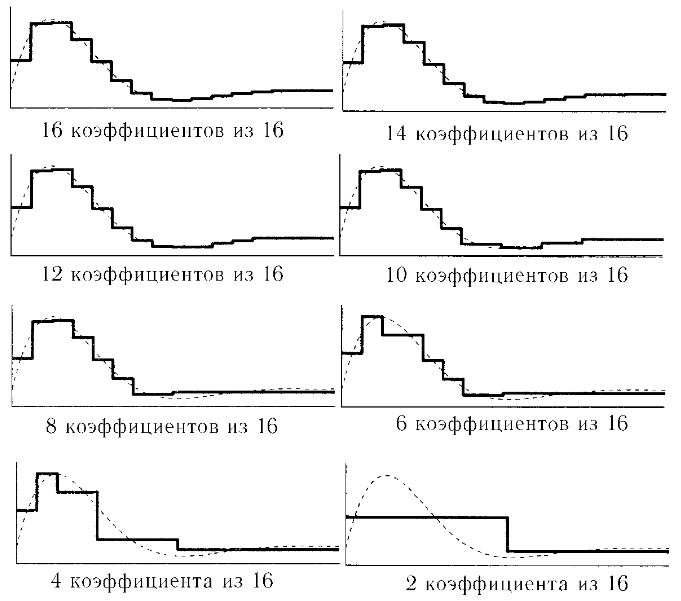
\includegraphics[scale=0.4]{inc/graphics/dec.png}
  \caption{Преобразование одномерной функции в коэффициенты с использованием функции нормированного базиса Хаара}
  \label{fig:dec}
\end{figure}

\subsection{Матричное представление DWT}
Пусть $v_{j}$ – последовательность конечной длины $c_{j,n}$ для некоторого $J$. Этот вектор преобразуется в вектор $v_{j+1}$, содержащий последовательности $c_{j+1,n}$ 
и $d_{j,n}$, каждая из которой половинной длины. Преобразование может быть записано в виде матричного умножения $v_{j+1} = M_{j}v^{j}$, где матрица $M_{j}$ – 
квадратная и состоит из нулей и элементов $h_{n}$, является ортонормированной, и обратная ей матрица является транспонированной.
В формулах \ref{eq:dwt1} и \ref{eq:dwt2} представлен пример прямого и обратного преобразования для фильтра длиной $L=4$, последовательности длиной $N=8$, начального значения $j=0$.
\begin{equation}\label{eq:dwt1}
\begin{bmatrix} 
c_{10} \\ c_{11} \\c_{12} \\c_{13} \\d_{10} \\d_{11} \\d_{12} \\d_{13} \\
\end{bmatrix}
=
\sqrt{2}
\begin{bmatrix} 
h_{0} & h_{1} & h_{2} & h_{3} &       &       &       &       \\ 
      &       & h_{0} & h_{1} & h_{2} & h_{3} &       &       \\ 
      &       &       &       & h_{0} & h_{1} & h_{2} & h_{3} \\
h_{2} & h_{3} &       &       &       &       & h_{0} & h_{1} \\
h_{3} &-h_{2} & h_{1} &-h_{0} &       &       &       &       \\ 
      &       & h_{3} &-h_{2} & h_{1} &-h_{0} &       &       \\ 
      &       &       &       & h_{3} &-h_{2} & h_{1} &-h_{0} \\
h_{1} & h_{0} &       &       &       &       & h_{3} &-h_{2} 
\end{bmatrix}
\begin{bmatrix} 
c_{00} \\ c_{01} \\c_{02} \\c_{03} \\c_{04} \\c_{05} \\c_{06} \\c_{07} \\
\end{bmatrix}
\end{equation}

Выражения \ref{eq:cwt11} и \ref{eq:cwt12} – это один шаг DWT. Полное DWT заключается в итеративном умножении верхней половины вектора $v^{j+1}$ 
на квадратную матрицу $M_{j+1}$, размер которой $2^{d-j}$. Эта процедура может повторяться $d$ раз, пока длина вектора не станет равна единице \cite{Pup04}. 

\begin{equation}\label{eq:dwt2}
\begin{bmatrix} 
c_{00} \\ c_{01} \\c_{02} \\c_{03} \\c_{04} \\c_{05} \\c_{06} \\c_{07} \\
\end{bmatrix}
=
\sqrt{2}
\begin{bmatrix} 

h_{0} &       &       & h_{2} & h_{3} &       &       & h_{1} \\
h_{1} &       &       & h_{3} &-h_{2} &       &       &-h_{0} \\
h_{2} & h_{0} &       &       & h_{1} & h_{3} &       &       \\
h_{3} & h_{1} &       &       &-h_{0} &-h_{2} &       &       \\
      & h_{2} & h_{0} &       &       & h_{1} & h_{3} &       \\
      & h_{3} & h_{1} &       &       &-h_{0} &-h_{2} &       \\
      &       & h_{2} & h_{0} &       &       & h_{1} & h_{3} \\
      &       & h_{3} & h_{1} &       &       &-h_{0} &-h_{2} 

\end{bmatrix}
\begin{bmatrix} 
c_{10} \\ c_{11} \\c_{12} \\c_{13} \\d_{10} \\d_{11} \\d_{12} \\d_{13} \\
\end{bmatrix}
\end{equation}


\subsection{Построение фильтров Добеши}
В настоящее время разработаны различные вейвлет-функции, ориентированные для решения различных задач. 
В данной работе для рассмотрения выбраны вейвлеты Добеши, так как предполагается, что увеличение числа 
ненулевых моментов для $Psi$ приводит к лучшей сжимаемости \cite{Pup01}. Добеши были сконструированы ортонормированные вейвлеты с компактными носителями на бесконечной вещественной оси.

Для построения фильтров Добеши процесс декомпозиции может быть записан как $v^{j+1}=M_{j}v^{j}$. Из свойств M:

\begin{equation}\label{eq:dwt3}
M_{j}^{T}v^{j} M_{j} = I
\end{equation}

$I$ - единичная матрица. Рассмотрим фильтр длиной 4. Получим матрицу, аналогичную \ref{eq:dwt1}. Из равенства \ref{eq:dwt3} следует, что 
$h_{0}^{2} + h_{1}^{2} + h_{2}^{2} + h_{3}^{2} = 1/2$, $h_{0}h_{1} + h_{2}h_{3} = 1/2$.
Эта система не дает единственного решения для фильтра $h_{m}$. Если потребовать, чтобы высокочастотный фильтр имел два нулевых момента:
$h_{3} - h_{2} + h_{1} - h_{0} = 0$, $h_{3} - 2h_{2} + 3h_{1} - 4h_{0} = 0$,
тогда: $h_{0} = \frac{1+\sqrt{3}}{4\sqrt{2}}$, $h_{1} = \frac{3+\sqrt{3}}{4\sqrt{2}}$, $h_{2} = \frac{3-\sqrt{3}}{4\sqrt{2}}$, $h_{3} = \frac{1-\sqrt{3}}{4\sqrt{2}}$.
Эти коэффициенты определяют вейвлеты, называемые D4-вейвлетами Добеши. 
Все фильтры Добеши могут быть получены посредством этой процедуры. 
Для фильтра длиной $L=2N$ необходимо $N$ равенств относительно нулевых моментов для получения единственного решения. 
В общем случае решение может быть получено численно. 

В $D_{4}$-конструкции задействованы следующие последовательности:
\begin{equation}
\begin{split}
 p=a=\frac{1}{4\sqrt{2}}(1+\sqrt{3}, 3+\sqrt{3}, 3-\sqrt{3}, 1-\sqrt{3}), \\
 q=b=\frac{1}{4\sqrt{2}}(1-\sqrt{3}, -3+\sqrt{3}, 3+\sqrt{3}, -1-\sqrt{3})
 \end{split}
\end{equation}

Последовательность $p$ представляет ненулевые элементы каждого столбца $P^{j}$, тогда как последовательность $q$ содержит ненулевые 
элементы столбца $Q^{j}$. Аналогично, последовательности $a$ и $b$ представляют строки $A^{j}$ и $B^{j}$ соответственно.
Последовательность для вейвлет фильтра можно получить, если поменять порядок элементов в последовательности масштабирующих функций 
и изменить их знаки на противоположные. Такие последовательности носят название квадратурных зеркальных фильтров.

$D_{4}$-масштабирующая функция и $D_{4}$-вейвлет изображены на рисунке \ref{fig:d4}. Обе функции ассиметричны и всюду недифференцируемы,
хотя при этом они являются непрерывными. Эти базисные функции являются членами целого семейства базисов, полученных Добеши,
включающего базисы, гладкость которых возрастает с увеличением носителей базисных функций.

\begin{figure}[ht]
  \centering
% [width=0.5\textwidth] --- регулировка ширины картинки
  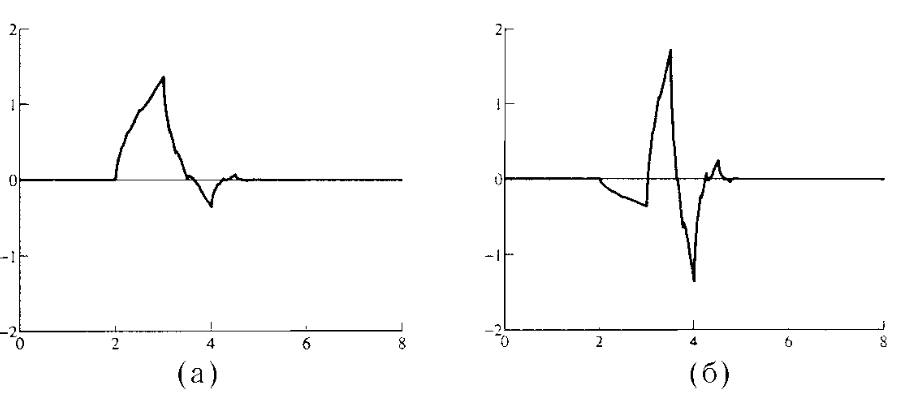
\includegraphics[scale=0.4]{inc/graphics/d4.png}
  \caption{Функции базиса вейвлетов Добеши: (а) $D_{4}$-масштабирующая функция; (б) $D_{4}$-вейвлет}
  \label{fig:d4}
\end{figure}

\subsection{Представление DWT для обработки двумерных и трехмерных данных}
Исходное изображение, например, один кадр из видео, может быть рассмотрено как одномерный массив, 
к которому затем применяется вейвлетное преобразование. 
В этом случае происходит перераспределение данных изображения, и не используется особенность избыточности данных изображений в двух измерениях. 
При применении вейвлетного преобразования к изображениям будем поочередно преобразовывать 
строки и столбцы исходного изображения, затем уменьшать рассматриваемую область в два раза. 
В начале рассматриваемая область соответствует всему изображению.
На рисунке \ref{fig:schema} представлена схема применения к изображению последовательности низкочастотных и высокочастотных фильтров. 
\begin{figure}[ht]
  \centering
% [width=0.5\textwidth] --- регулировка ширины картинки
  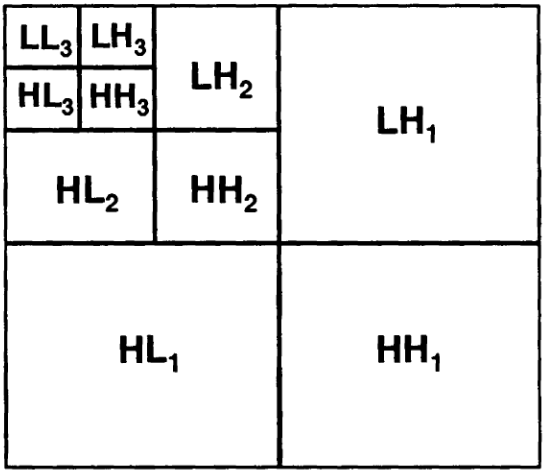
\includegraphics[scale=0.5]{inc/graphics/schema.png}
  \caption{Схема применения к изображению последовательности низкочастотных $L$ и высокочастотных $H$ фильтров. 
  На схеме $LH_{x}$ – вертикальное высокочастотное фильтрование, к которому применяется горизонтальное 
  низкочастотное фильтрование, $HL_{x}$ – вертикальное низкочастотное фильтрование, 
  к которому применяется горизонтальное высокочастотное фильтрование}
  \label{fig:schema}
\end{figure}
Обозначим высокочастотный фильтр $H$, а низкочастотный фильтр $L$. Тогда $LH_{x}$ – 
вертикальное высокочастотное фильтрование, к которому применяется горизонтальное 
низкочастотное фильтрование, $HL_{x}$ – вертикальное низкочастотное фильтрование, 
к которому применяется горизонтальное высокочастотное фильтрование \cite{Pup03}.
При обратном вейвлет-преобразовании к данным применяется та же последовательность действий в обратном порядке.

Для использования кратномасштабного анализа при обработке видео необходимо реализовать 3D-версию 
анализа и синтеза банков фильтров. В случае трехмерного преобразования вейвлет преобразование применяется к 
каждому из трех измерений. Если данные имеют размеры $N_{1} \times N_{2} \times N_{3}$, то применение вейвлет преобразования к первому измерению
дает два набора данных, каждый из которых имеет размер $N_{1} / 2 \times N_{2} \times N_{3}$. 
Применение вейвлет преобразования ко второму измерению дает четыре набора данных, 
каждый из которых имеет размер $N_{1} / 2 \times N_{2} / 2 \times N_{3}$. Применение вейвлет преобразования 
к третьему измерению дает восемь наборов данных, каждый из которых имеет размер $N_{1} / 2 \times N_{2} / 2 \times N_{3} / 2$. 
Это показано на рисунке \ref{fig:fig01}, где $X$ - исходный набор данных, $W$ - набор данных после применения вейвлет преобразования,
индекс $L$ - набор данных после применения низкочастотного фильтра, индекс $H$ - набор данных после применения высокочастотного фильтра.

\begin{figure}[ht]
  \centering
% [width=0.5\textwidth] --- регулировка ширины картинки
  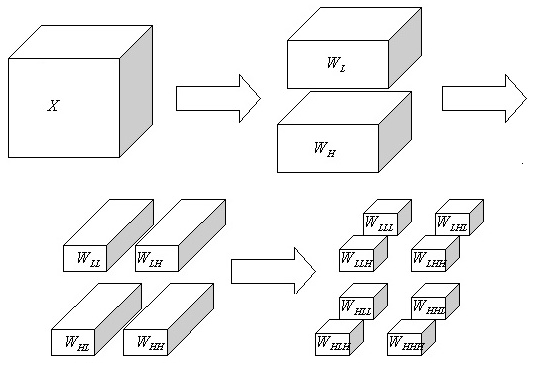
\includegraphics[scale=0.75]{inc/graphics/3dwave.png}
  \caption{Схема применения к трехмерным данным последовательности низкочастотных $L$ и высокочастотных $H$ фильтров, где $X$ - исходный набор данных, $W$ - набор данных после применения вейвлет преобразования,
индекс $L$ - набор данных после применения низкочастотного фильтра, индекс $H$ - набор данных после применения высокочастотного фильтра}
  \label{fig:fig01}
\end{figure}

\section{Достоинства и недостатки вейвлет-преобразований}
\begin{itemize}
 \item Вейвлет-преобразования обладают всеми достоинствами преобразования Фурье
 \item Вейвлетные базисы могут быть хорошо локализованными как по частоте, так и по времени. 
 При выделении в сигналах разномасштабных процессов можно рассматривать выбранные масштабные уровни разложения
 \item Вейвлетные базисы имеют разнообразные базовые функции, свойства которых ориентированы на решение различных задач
 \item Недостатком вейвлет-преобразований является их относительная сложность
\end{itemize}

\section{Метрики оценки качества видео}

Наиболее часто используемые сравнительные оценки качества двух изображений – 
это среднеквадратическая ошибка и пиковое отношение сигнал-шум. 
Методы, основанные на этих оценках, хороши для изображений, имеющих 
белый шум. Однако эти меры некорректно отражают структурные искажения при 
кодировании (сжатии), а также плохо коррелируют с визуальной оценкой 
качества. 

Важнейшими характеристиками при сравнении различных методов
кодирования видео сигналов является выходной битрейт и оценки качества
восстановленного после декодирования видео потока. 
Одним из простых критерием оценки потери качества является
среднеквадратическое отклонение значений пикселей сжатого изображения от
оригинала.
По этому критерию изображение будет сильно испорчено при изменении
яркости всего на 5\%. В тоже время изображение со снегом, резким изменением
цвета отдельных точек будут признаны почти не изменившимися.
Другим критерием является максимальное отклонение от оригинала.
Даная мера крайне чувствительна к биению отдельных пикселей, т.е. в
изображении может измениться только один пиксель, и данный критерий
признает изображение сильно испорченным.
На практике используемой мерой качества изображения является
критерий соотношения сигнал/шум (PSNR). Эта мера аналогична
среднеквадратическому отклонению, но пользоваться ей удобнее из-за
логарифмического масштаба шкалы.
Лучше всего потери в качестве оценивает человеческий глаз. Сжатие
изображение можно считать отличной, если на глаз невозможно отличить
оригинал от сжатого изображения. Но на практике при сжатии с потерями в
изображение всегда вносятся какие-либо искажения заметные при сравнении
оригинала и сжатого изображения.
Среди большого числа критериев оценки качества восстановленного
изображения наибольшее распространение получили среднеквадратическое
отклонение и соотношение сигнал/шум, а для визуальной оценки используется
разностное изображение.
На практике, видео изображение со значениями PSNR порядка 40-43 дБ и
выше является изображением очень высокого качества. Сжатое изображение с
уровнем PSNR свыше 43 дБ в связи с особенностями человеческого зрения
неотличимо от оригинала, с уровнем от 40 до 43 дБ показывает отличное
качество изображения, с уровнем PSNR от 35 до 40 дБ – хорошее, от 30 до 35
дБ - приемлемое качество изображения, с уровнем PSNR ниже 30 дБ –
неприемлемое качество изображения \cite{Pup02}.

\subsection{PSNR}

Метрика, которую часто используют на практике, называется мерой отношения сигнала 
к шуму (peak-to-peak signal-to-noise ratio — PSNR).

\begin{equation}\label{eq:psnr}
PSNR = 10\log_{10}\frac{MaxErr^{2}wh}{\sum_{i = 0, j = 0}^{w,h}(x_{i,j}-y_{i,j})^2}
\end{equation}

PSNR рассчитывается по формуле \ref{eq:psnr} где MaxErr - максимум модуля разности цветовой компоненты, w - ширина видео, h - высота видео. 
Данная метрика, по сути, аналогична среднеквадратичному отклонению, однако пользоваться ей несколько удобнее за счет логарифмического масштаба шкалы. 
Ей присущи те же недостатки, что и среднеквадратичному отклонению.

\subsection{MSAD}

Значением данной метрики является усреднённая абсолютная разность значений цветовых компонент 
в соответствующих точках сравниваемых изображений. 
Используется, например, для отладки кодеков или фильтров. Расчитывается по формуле \ref{eq:msad}

\begin{equation}\label{eq:msad}
d(X,Y)= \frac{\sum_{i = 1, j = 1}^{m,n}\Bigl|X_{i,j}-Y_{i,j}\Bigr|}{mn}
\end{equation}

\subsection{SSIM INDEX}

Индекс структурного сходства (от англ. SSIM - structure similarity) является одним 
из методов измерения схожести между двумя изображениями. SSIM индекс это метод 
полного сопоставления, другими словами, он проводит измерение качества на 
основе исходного изображения (не сжатого или без искажений). SSIM индекс 
является развитием традиционных методов, таких как PSNR и метод среднеквадратичной 
ошибки MSE, которые оказались несовместимы с физиологией человеческого восприятия.
Отличительной особенностью метода, помимо упомянутых ранее (MSE и PSNR), является 
то, что метод учитывает "восприятие ошибки", благодаря учёту структурного изменения 
информации. Идея заключается в том, что пиксели имеют сильную взаимосвязь, 
особенно когда они близки пространственно. Данные зависимости несут важную информацию о 
структуре объектов и о сцене в целом.
SSIM метрика рассчитана на различные размеры окна. 
Разница между двумя окнами x и y имеющими одинаковый размер $N \times N$. Расчитывается по формулам 
\ref{eq:ssim}

\begin{equation}\label{eq:ssim}
SSIM= \Bigl(  \frac{2\sigma_{x}\sigma_{y}}{\sigma_{x}^{2}+\sigma_{y}^{2}} \Bigr) 
\Bigl( \frac{2\bar{X}\bar{Y}}{ \bigl( \bar{X} \bigr) ^{2} + \bigl( \bar{Y} \bigr) ^{2} } \Bigr)
\Bigl(  \frac{\sigma_{xy}}{\sigma_{x}\sigma_{y}} \Bigr); 
\end{equation}
\begin{equation}\label{eq:ssim1}
\begin{split}
\bar{X}=\frac{1}{MN}\sum_{i=1}^{M}\sum_{j=1}^{N}x_{ij},\bar{Y}=\frac{1}{MN}\sum_{i=1}^{M}\sum_{j=1}^{N}y_{ij}; \\
\sigma_{x}^2=\frac{1}{(M-1)(N-1)}\sum_{i=1}^{M}\sum_{j=1}^{N}(x_{ij}-\bar{X})^2; \\
\sigma_{y}^2=\frac{1}{(M-1)(N-1)}\sum_{i=1}^{M}\sum_{j=1}^{N}(y_{ij}-\bar{Y})^2; \\
\sigma_{xy}=\frac{1}{(M-1)(N-1)}\sum_{i=1}^{M}\sum_{j=1}^{N}(x_{ij}-\bar{X})(y_{ij}-\bar{Y}), 
\end{split}
\end{equation}

где SSIM – значение меры сходства (качества) изображений; $X=\{x_{ij}\}$ и $Y=\{y_{ij}\}$ – 
сравниваемые изображения; $M$, $N$ – размеры изображения. Первая составляющая 
выражения \ref{eq:ssim} является коэффициентом корреляции между изображениями X и Y. 
Вторая составляющая характеризует сходство средних значений яркостей двух сравниваемых изображений. 
Третья составляющая характеризует сходство контрастов 
двух сравниваемых изображений. 

Чем выше значение меры сходства изображений, тем лучше выполнена обработка изображения. 
В общем случае мера сходства изображений рассчитывается в 
непересекающихся областях для каждого изображения отдельно. Поскольку на изоб-
ражениях сцены объекты не изменялись и не двигались, меру можно вычислять сразу 
на всем изображении. 

\section{Метод сжатия видео на основе кратномасштабного анализа}

В разрабатываемой системе необходимо выделить параметры, которые влияют на поведение системы.
Были выделены следующие параметры:
\begin{itemize}
 \item Размер блока
 \item Порядок системы коэффициентов для вейвлетного преобразования
 \item Процент сохраняемых данных
 \item Алгоритм кодирования без потерь
\end{itemize}
Эти параметры передаются как входные данные вместе с графическими данными.

Вейвлетное преобразование является эффективным, если имеется избыточность графических данных \cite{Pup11}. Для трехмерного вейвлетного преобразования, в частности,
преобразования блоков в видео, необходима избыточность в трех измерениях. Это означает что соседние пиксели на одном кадре и на смежных кадрах должны иметь одинаковое 
или близкое значение цветовых компонент. 

Для определения избыточности на видео необходимо провести предварительный анализ графических данных. На видео необходимо найти такие блоки,
где избыточность во всех трех измерениях будет максимальной. Такие блоки могут быть выделены следующим образом. На видео необходимо найти смены сцен и планов.
План - это система условного деления кинематографического пространства (то есть пространства, представленного на экране). 
Предполагается, что избыточность в данных будет присутствовать только пока последовательность кадров представляет один и тот же план. Как только происходит смена плана,
в данных между кадрами наблюдается резкая граница, которая требует дополнительной информации при кодировании.
Таким образом, во время анализа данных необходимо найти смены планов. Каждая смена означает границу определенного блока.

Для поиска границ между блоками необходимо определить способ сравнения кадров. Для этой задачи могут быть использованы метрики оценки качества видео, описанные ранее,
такие как PSNR, MSAD, SSIM INDEX.

Необходимо также определить минимальный размер блока и максимальный размер блока. Минимальный размерблока требуется для устранения большого количество блоков
малого размера, что посребует вычислительных ресурсов для их обработки.
Максимальный размер блока определяется мощностью машины, на которой производятся вычисления.

Для поиска границ между блоками будем последовательно просматривать кадры видео и вычислять разницу между соседними кадрами по одной из метрик. 
Определим некоторое пороговое значение $\sigma$, превышение этого значения при вычислении разницы между кадрами будет означать 
наличие границы между блоками. Общая схема поиска блоков на видео представлена на рисунке \ref{fig:figblocks}. 



Преобразование видео с использованием вейвлетных преобразований состоит из двух основных этапов – 
прямого преобразования и обратного преобразования, общая схема представлена на рисунке \ref{fig:figalg}. 
Последовательное применение прямого и обратного преобразований не изменяет данные.
Прямое преобразование с последующим квантованием и децимацией позволяет сжать
исходные данные. Качество видео при этом зависит от параметров кодирования.

\begin{figure}[ht]
  \centering
% [width=0.5\textwidth] --- регулировка ширины картинки
  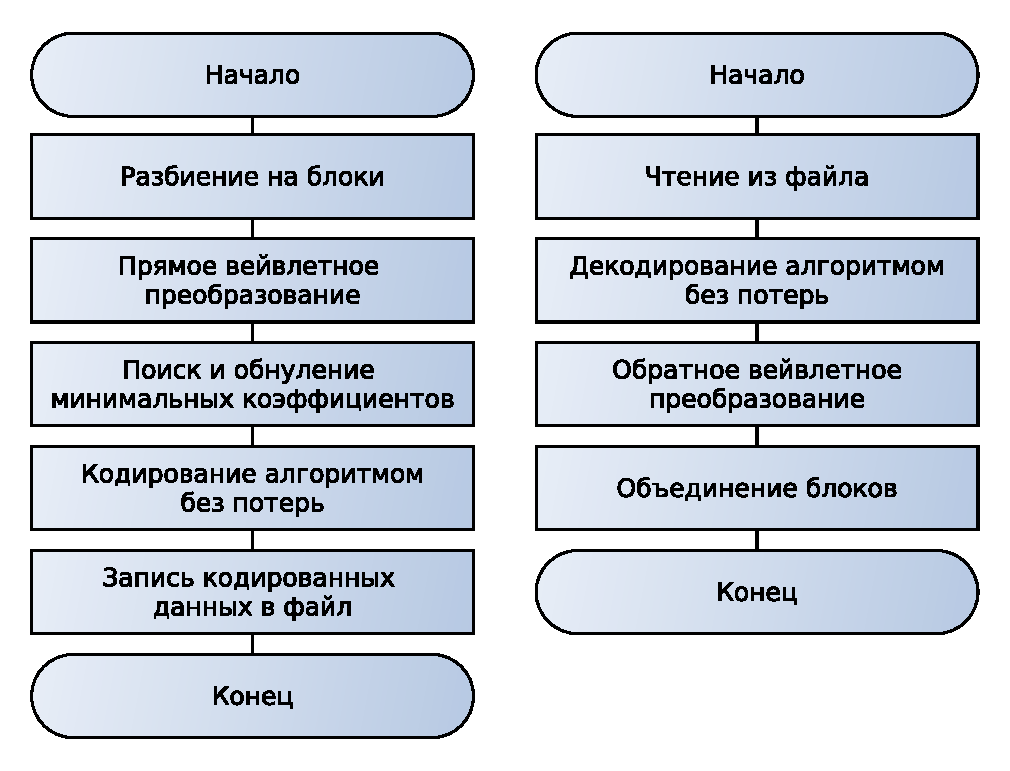
\includegraphics[scale=0.75]{inc/graphics/alg.pdf}
  \caption{Общая схема компрессии и декомпрессии видео}
  \label{fig:figalg}
\end{figure}

Вейвлетное преобразование для данных в третьем измерении, то есть для видео по времени, требует
разбиения видео на блоки по кадрам. Это необходимо, так как видео, как правило, содержит большое число кадров. 
Это означает, что вейвлетное преобразование видео по времени потребует большое количесво вычислительных ресурсов.
После разбиения на блоки необходимо применить вейвлет преобразование к каждому блоку в трех измерениях.

После применения вейвлет преобразования к блоку будет получен блок данных, содержащий
информацию о высоких и низких частотах в блоке. Применение обратного преобразования на этом этапе
позволит получить исходный набор данных.

Далее необходимо провести децимацию данных в преобразованном блоке. 
Перед началом работы пользователем определяется процент данных, который будет удален из каждого блока.
Для проведения децимации необходимо найти все минимальные коэффициенты и обнулить их. Их количество 
должно соответствовать указанному проценту удаляемых данных.
Блок данных после децимации содержит нули и может быть закодирован. При достаточно большом количестве нулевых данных
могут использоваться специальные структуры данных для хранения разреженных данных. 
Далее необходимо сжать получившиеся данные с помощью алгоритмов сжатия без потерь. Это позволяет
максимально уменьшаеть объем памяти, занимаемый итоговым файлом на диске, однако уменьшает скорость декомпрессии. 

Для воспроизведения видео необходимо провести действия в обратном порядке. 
Сначала необходимо провести декомпрессию преобразованных данных выбранным алгоритмом сжатия без потерь.
Затем к каждому преобразованному блоку необходимо применить обратное вейвлетное преобразование. 
После чего блоки должны быть объединены в общую последовательность кадров.

\begin{figure}[ht]
  \centering
% [width=0.5\textwidth] --- регулировка ширины картинки
  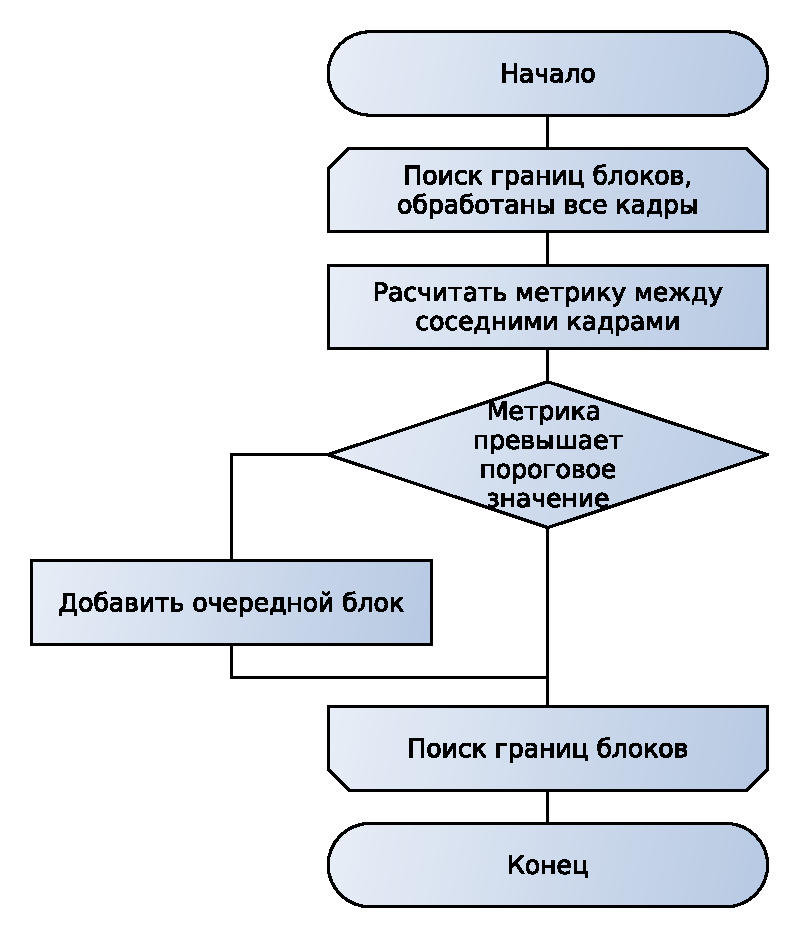
\includegraphics[scale=0.75]{inc/graphics/method1.pdf}
  \caption{Схема поиска блоков на видео}
  \label{fig:figblocks}
\end{figure}


\chapter{Конструкторский раздел}
\label{cha:design}

\section{Требования к разрабатываемому программному обеспечению}
К разрабатываемому программному обеспечению предъявляются следующие высокоурованевые требования:
\begin{itemize}
 \item разрабатываемое программное обеспечение должно обеспечивать функционирование по требованию пользователя,
 \item программное обеспечение должно производить кодирование и декодирование указанного файла с графическими данными,
 \item программное обеспечение должно проводить анализ графических данных и осуществлять разбиение графических данных на блоки,
 \item программное обеспечение должно выполнять прямое и обратное вейвлетное преобразование блоков графических данных,
 \item программное обеспечение должно выполнять децимацию графических данных после применения вейвлетного преобразования.
\end{itemize}

\section{Пользовательские требования к программному обеспечению}
Пользовательские требования (функциональные требования с точки зрения пользователей) описывают цели и задачи пользователей
программного обеспечения, которые должны достигаться и выполняться пользователями при помощи разрабатываемого программного обеспечения.
К разрабатываемому программному обеспечению предъявляются следующие требования:
\begin{itemize}
 \item разрабатываемое программное обеспечение должно позволять пользователю выбирать файл с графическими данными,
 \item программное обеспечение должно позволять пользователю задавать процент сохраняемых данных,
 \item программное обеспечение должно позволять пользователю выполнять кодирование файла с графическими данными с помощью разработанного метода 
 с использованием кратномасштабного анализа,
 \item программное обеспечение должно позволять пользователю выполнять декодирование файла с преобразованными графическими данными,
 \item программное обеспечение должно выполнить воспроизведение графических данных после декодирования.
\end{itemize}

\section{Входные и выходные параметры}
Разрабатываемое программное обеспечение состоит из двух частей:
\begin{itemize}
 \item кодирование графических данных,
 \item декодирование графических данных.
\end{itemize}
Входными данными для функционала кодирования графических данных являются исходный файл с графическими даннными и процент сохраняемых данных.
Выходными данными для функционала кодирования графических данных является файл, содержащий кодированную последовательность графических данных после
применения вейвлетного преобразования и децимации.
Входными данными для функционала декодирования графических данных являются исходный файл с кодированными графическими даннными.
Выходными данными для функционала декодирования графических данных является последовательность кадров, состоящая из графических данных, полученных после применения 
обратного вейвлетного преобразования.

\section{Сценарии функционирования}
Сценарии функционирования разрабатываемого программного комплекса представлены на рисунке \ref{fig:uml1}.

\begin{figure}[ht]
  \centering
  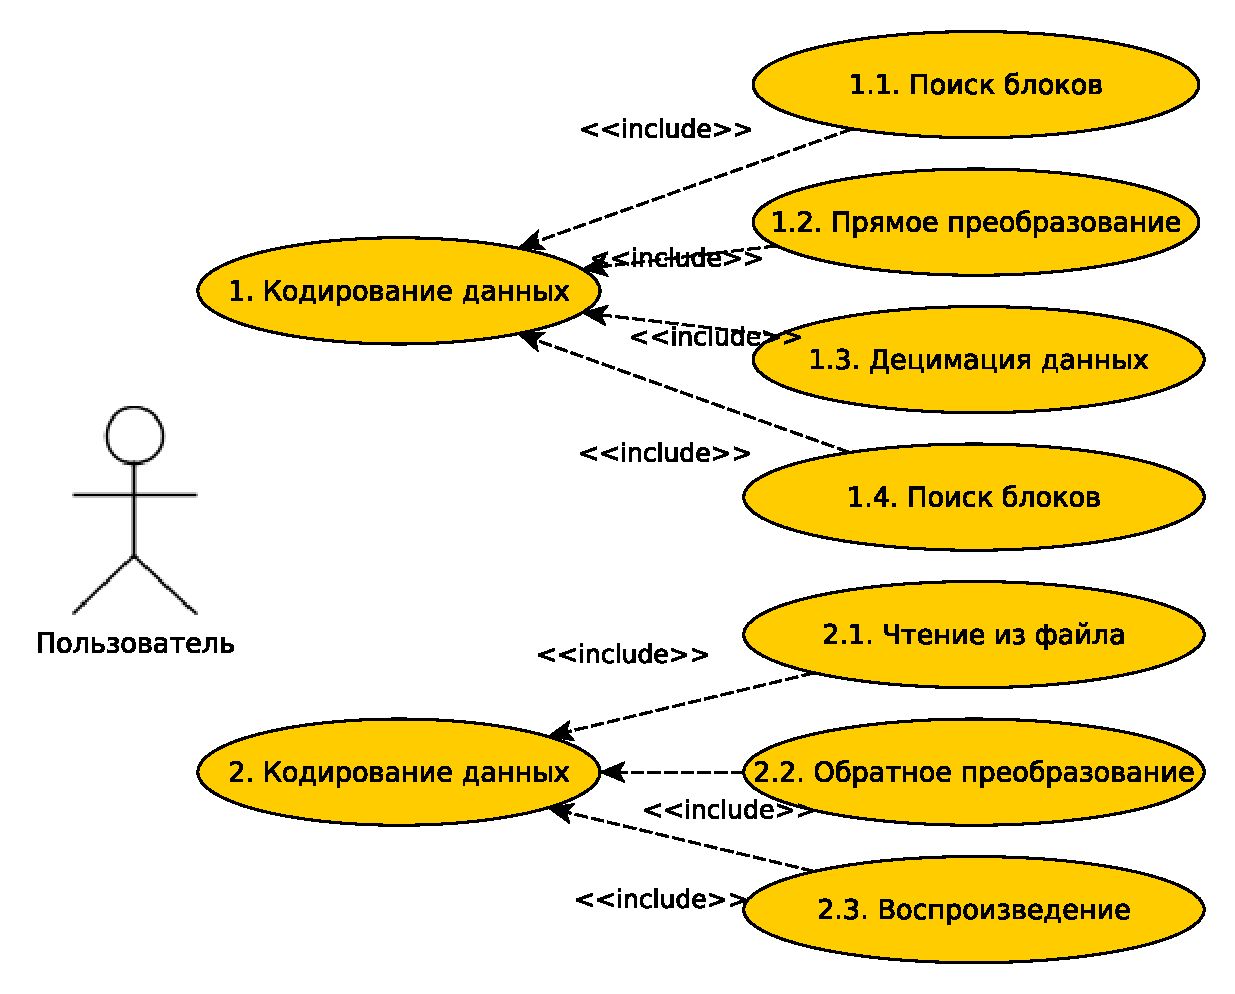
\includegraphics[scale=0.65]{inc/graphics/uml1.pdf}
  \caption{Диаграмма вариантов использования с точки зрения пользователя}
  \label{fig:uml1}
\end{figure}

Возможны следующие сценарии использования программного обеспечения:
\begin{itemize}
 \item Прецедент 1 - Кодировать данные
    \subitem Прецедент 1.1 - Анализ графических данных и поиск блоков
    \subitem Прецедент 1.2 - Прямое вейвлетное преобразование
    \subitem Прецедент 1.3 - Децимация графических данных
    \subitem Прецедент 1.4 - Запись кодированных данных в файл
 \item Прецедент 2 - Декодировать данные
    \subitem Прецедент 2.1 - Чтение графических данных из файла
    \subitem Прецедент 2.2 - Обратное вейвлетное преобразование
    \subitem Прецедент 2.3 - Воспроизведение видео
\end{itemize}



\section{Алгоритм сжатия видео с использованием кратномасштабного анализа}
В соответствии со схемой \ref{fig:figalg} прямого и обратного преобразования был разработан алгоритм сжатия видео.

В разрабатываемой системе важна скорость сжатия. Поэтому для разбиения на блоки использовалась 
усредненная абсолютная разность значений цветовых компонент, так как для ее определения необходимо наименьшее количество вычислений.

Для вейвлетного преобразования необходимо выделить параметры, которые влияют на поведение системы.
Были выделены следующие параметры:
\begin{itemize}
 \item Размер блока
 \item Порядок системы коэффициентов для вейвлетного преобразования
 \item Процент сохраняемых данных
 \item Алгоритм кодирования без потерь
\end{itemize}
Эти параметры передаются как входные данные вместе с графическими данными.

В разрабатываемой системе для выполнения вейвлет-преобразования необходимо разработать отдельный модуль. 
Для прямого и обратного преобразований необходимо получить систему вейвлет-коэффициентов нужного порядка. 
Для этого необходимо разработать функции получения набора коэффициентов указанной системы коэффициентов. 

Для алгоритма прямого преобразования необходимо инициализировать размер рассматриваемой области. 
В начале работы алгоритма размер рассматриваемой области равен размеру блока. 
В процессе работы алгоритма размер рассматриваемой области уменьшается. 
Если ширина, высота, глубина рассматриваемой области равны единице, то необходимо закончить вейвлет-преобразование. 

На каждой итерации вейвлет-преобразование применяется ко всем векторам рассматриваемой области 
блока сначала по ширине, затем по высоте, затем по глубине, ширина, высота и глубина рассматриваемой области уменьшаются в два раза. 
Для выполнения вейвлет-преобразования необходимо составить матрицу вейвлет-преобразования в соответствии с 
размером рассматриваемой области. 
Прямое вейвлет-преобразование может быть реализовано как рекурсивно, так и итеративно. 
Подробная схема разработанного алгоритма прямого вейвлет-преобразования представлена на рисунке \ref{fig:figalgdir}. 
Код процедуры прямого вейвлетного преобразования блока представлен в листинге \ref{lst:dir}, где \texttt{block} - графические данные, которые необходимо преобразовать,
\texttt{block\_size} - количество кадров в блоке, \texttt{с} - количество каналов в блоке, \texttt{h} - высота блока, \texttt{w}
- ширина блока, \texttt{s} - система коэффициентов, \texttt{p} - процент 
сохраняемых данных.

\begin{figure}
  \centering
% [width=0.5\textwidth] --- регулировка ширины картинки
  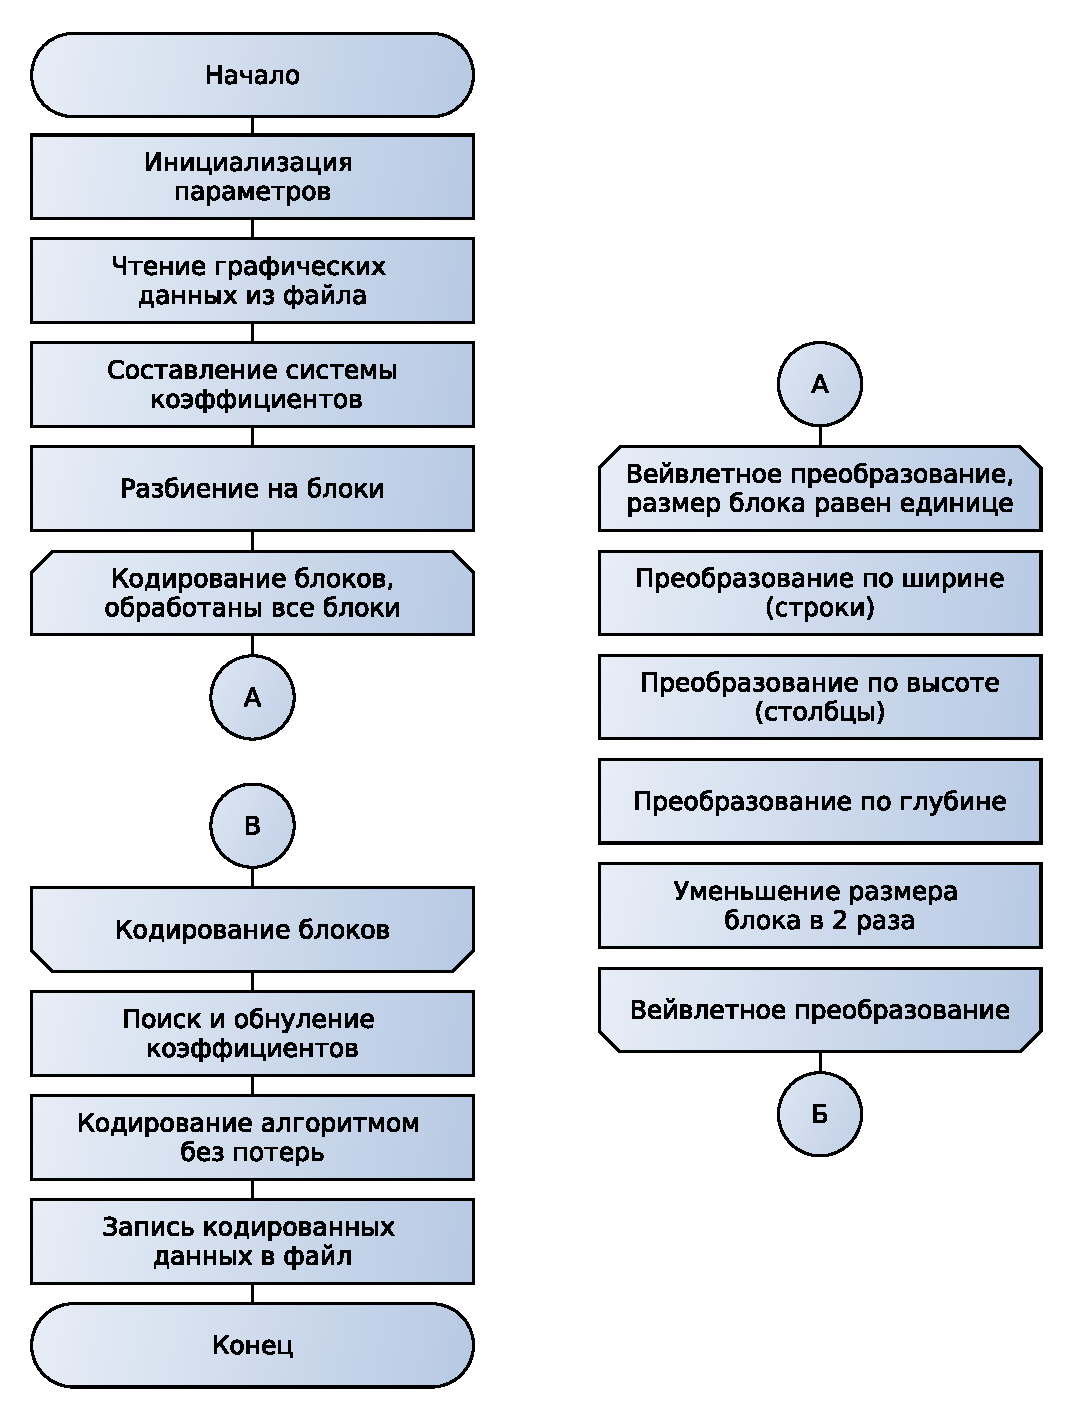
\includegraphics[scale=0.75]{inc/graphics/alg1.pdf}
  \caption{Cхема компрессии видео}
  \label{fig:figalgdir}
\end{figure}

\begin{lstlisting}[style=pseudocode,caption={Код процедуры transform\_block},label=lst:dir]
transform_block(block, block_size, c, h, w, s, p)
  block_data := CopyBlockData(block, block_size, c, h, w)
  DirectTransform(block_data, c, w, h, block_size, w, h, block_size, s)
  out_data := Decimate(block_data, c, w, h, block_size, p)
  FreeBlockData(block_data, block_size, c, h, w)
  return out_data
\end{lstlisting}
   
Для алгоритма обратного преобразования необходимо рассчитать размер рассматриваемой области, 
так как блок может иметь разные размеры по высоте, ширине и глубине. В процессе работы алгоритма 
размер рассматриваемой области увеличивается. Если ширина и высота рассматриваемой области 
соответствуют размерам изображения, то необходимо закончить обратное вейвлет-преобразование.
Подробная схема разработанного алгоритма обратного вейвлет-преобразования представлена на рисунке \ref{fig:figalg2}.
Код процедуры обратного вейвлетного преобразования блока представлен в листинге \ref{lst:back}, где \texttt{out\_data} - кодированные данные, к которым 
необходимо применить обратное вейвлетное преобразование,
\texttt{block\_size} - количество кадров в блоке, \texttt{с} - количество каналов в блоке, \texttt{h} - высота блока, \texttt{w}
- ширина блока, \texttt{s} - система коэффициентов

\begin{lstlisting}[style=pseudocode,caption={Код процедуры decode\_block},label=lst:back]
decode_block(out_data, block_size, c, h, w, system)
  block_data = AllocateBlock(block_size, c, h, w)
  ConvertArrayToMatrix(out_data, block_data)
  InverseTransform(block_data, c, w, h, block_size, w, h, block_size, system)
  block = AllocateFrames(block_size, c, h, w)
  for int i := 0; i < block_size; ++i
    block[i] = WriteImageData(block_data[i])
  FreeBlockData(block_data, block_size, c, h, w)
  return block
\end{lstlisting}


\begin{figure}
  \centering
  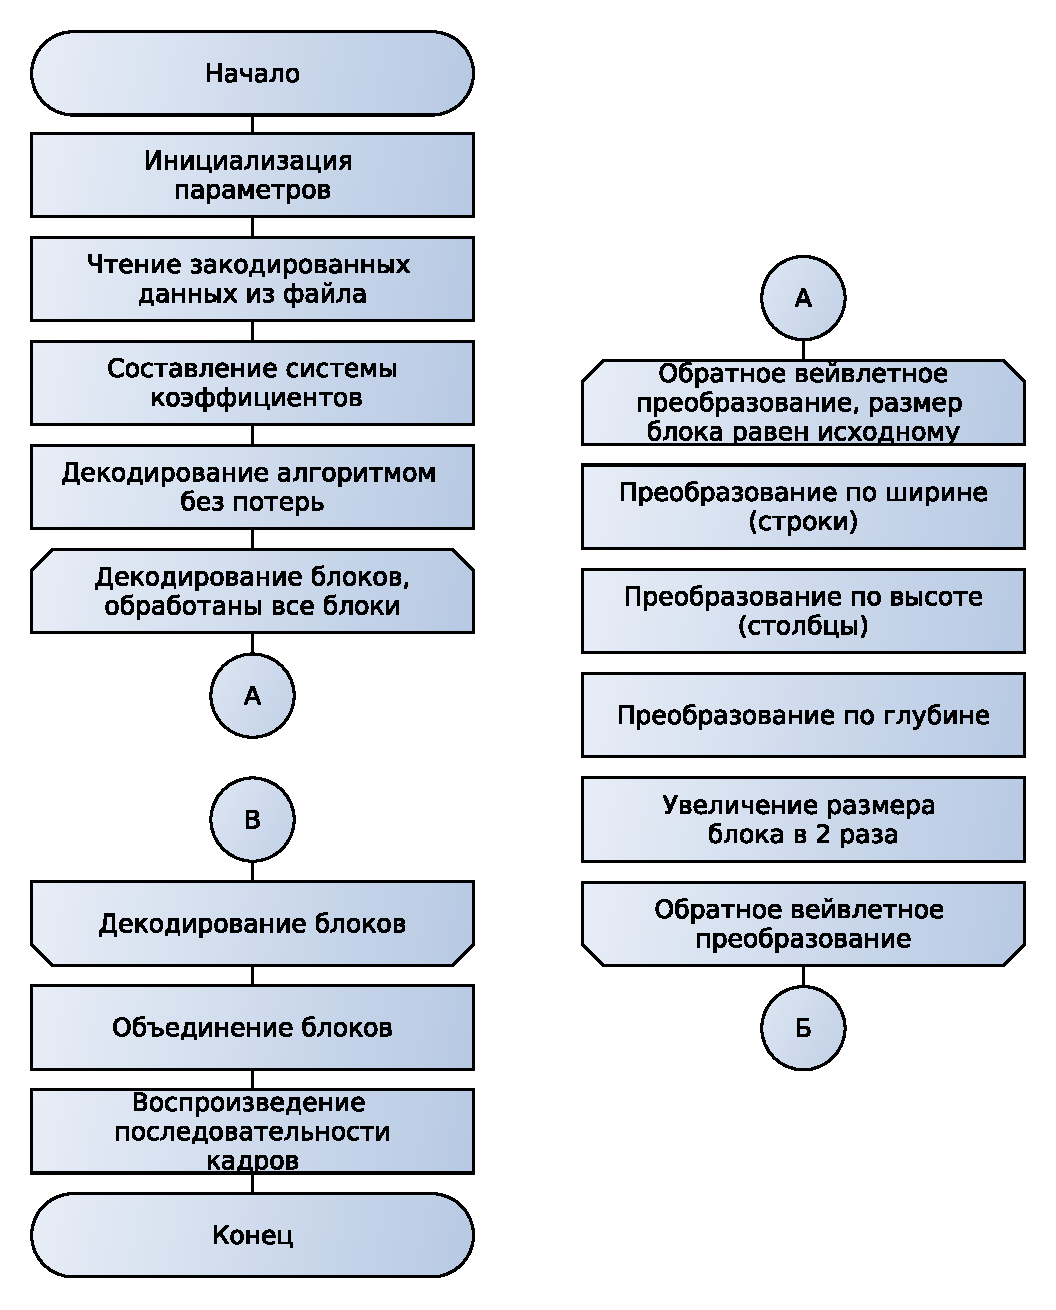
\includegraphics[scale=0.75]{inc/graphics/alg2.pdf}
  \caption{Cхема компрессии видео}
  \label{fig:figalg2}
\end{figure}


\section{Составление матриц}
В данной работе для рассмотрения выбраны вейвлеты Добеши, так как предполагается, 
что увеличение размера системы коэффициентов приводит к лучшей сжимаемости \cite{Pup01}.
Матрица прямого преобразования M состоит из двух прямоугольных матриц L и H,  
представляющих низкочастотный и высокочастотный фильтры. Матрицы L и H могут быть составлены следующим образом:
\begin{equation}
L= \begin{cases}
 c_{j-2i+1+n}, \mbox{при $j-2i+1<0$} \\
 c_{j - 2i + 1}, \mbox{иначе}
\end{cases}
\label{F:F2}
\end{equation}
\begin{equation}
L= \begin{cases}
 (-1)^{j+1}c_{2i-j+n}, \mbox{при $2i-j<0$} \\
 (-1)^{j+1}c_{2i-j}, \mbox{иначе}
\end{cases}
\label{F:F2}
\end{equation}              
Матрица обратного преобразования является транспонированной матрицей прямого преобразования. Код процедуры заполнения 
матрицы преобразования представлен в листинге \ref{lst:PrepareMatrix}, где m - матрица преобразования, dim - размерность матрицы
преобразования, system - выбранная система коэффициентов.
        
\begin{lstlisting}[style=pseudocode,caption={Код процедуры PrepareMatrix},label=lst:PrepareMatrix]
PrepareMatrix(m, dim, system)
  if dim % 2 != 0
    then dim := dim - 1
  i := 0
  j := 0
  for i := 0; i < dim / 2; ++i
    for j := 0; j < dim; ++j)
      index := (j + 1) - 2 * (i + 1) + 1
      system_index := index < 0 ? index + dimension : index
      m[i][j] := system_index >= 0 && system_index < system.size ? system[system_index] : 0
      
  for i := 0; i < dim / 2; ++i)
    for j := 0; j < dim; ++j
      index := 2 * (i + 1) - (j + 1);
      system_index := index < 0 ? index + dimension : index
      if system_index < 0 or system_index >= system.size()
        then m[i + dim / 2][j] := 0
        else
          if (j + 2) % 2 != 0
            then m[i + dim / 2][j] = -system[system_index]
            else m[i + dim / 2][j] = system[system_index]
\end{lstlisting}

\section{Поиск и обнуление минимальных коэффициентов после применения вейвлет-преобразования}
После применения прямого вейвлетного преобразования необходимо обеспечить 
сжатие путем обнуления части коэффициентов. Степень сжатия задается 
пользователем в процентах. Из ненулевых элементов необходимо выбрать указанный пользователем процент 
максимальных элементов. Это значит, что необходимо найти указанную пользователем 
порядковую статистику в наборе графических данных. 
Видео содержит большое количество кадров, каждый кадр содержит несколько каналов, 
массив графических данных может содержать по несколько тысяч элементов. 
Поэтому необходимо производить эффективный поиск порядковой статистики. Рассмотрим 
алгоритм, выполняющий поиск порядковой статистики за линейное время $O(n)$, где $n$ - 
размерность входных данных для поиска порядковой статистики.
Заранее не известно количество ненулевых элементов в массиве, 
для определения номера искомой порядковой статистики необходимо подсчитать количество ненулевых элементов. 
Зная это количество и указанный пользователем процент, точно определяется номер искомой порядковой статистики. 

Алгоритм \texttt{Randomized\_Select} поиска порядковой статистики разработан по аналогии 
с алгоритмом быстрой сортировки. Как и в алгоритме быстрой сортировки, в алгоритме 
\texttt{Randomized\_Select} используется идея рекурсивного разбиения входного массива. 
В отличие от алгоритма быстрой сортировки, в котором рекурсивно обрабатываются обе части разбиение, 
алгоритм \texttt{Randomized\_Select} работает лишь с одной частью. Это различие проявляется 
в результатах анализа обоих алгоритмов: если математическое ожидание времени работы
алгоритма быстрой сортировки равно $\Theta(n \lg n)$, то ожидаемое время работы алгоритма 
\texttt{Randomized\_Select} равно $\Theta(n)$, в предположении, что все элементы входных множеств различны.

В алгоритме \texttt{Randomized\_Select} используется процедура Randomized\_Partition. 
Подобно быстрой сортировке, \texttt{Randomized\_Select} – рандомозированный алгоритм, 
поскольку его поведение частично определяется выводом генератора случайных чисел. 
Код процедуры \texttt{Randomized\_Select} представлен в листинге \ref{lst:RandomizedSelect}, где входные параметры A – Массив данных,
p – левая граница части массива для поиска,
r – правая граница части массива для поиска,
i – номер искомой порядковой статистики, возвращаемое значение это искомая порядковая статистика.

        
\begin{lstlisting}[style=pseudocode,caption={Код процедуры Randomized\_Select},label=lst:RandomizedSelect]
Randomized_Select(A, p, r, i) 
  if p = r 
    then return A[p] 
  q := Randomized_Partition(A, p, r) 
  k := q - p + 1
  if i = k
    then return A[q]
  else if i < k
    then return Randomized_Select(A, p, q - 1, i)
  else return Randomized_Select(A, q + 1, r, i - k)
\end{lstlisting}
        
После выполнения процедуры \texttt{Randomized\_Partition}, которая вызывается  в строке 4 
представленного выше алгоритма, массив \texttt{А[р..r]} оказывается разбитым на два (возможно, пустых) 
подмассива \texttt{A[p..q-1]} и \texttt{A[q+l..r]}. При этом величина каждого элемента \texttt{A[p..q-1]} не превышает 
\texttt{A[q]}, а величина каждого элемента \texttt{А[q+1..r]} больше \texttt{A[q]}. 
Как и в алгоритме быстрой сортировки, элемент \texttt{A[q]} будем называть опорным (\texttt{pivot}). 
В строке 5 процедуры \texttt{Randomized\_Select} вычисляется количество элементов \texttt{k} подмассива \texttt{А[p..q]}, 
то есть количество элементов, попадающих в нижнюю часть разбиения плюс один опорный элемент. 
Затем в строке 6 проверяется, является ли элемент \texttt{A[q]} \texttt{i}-м в порядке возрастания элементом. 
Если это так, то возвращается элемент \texttt{A[q]}. В противном случае в алгоритме определяется, в 
каком из двух подмассивов содержится \texttt{i}-й в порядке возрастания элемент: в подмассиве \texttt{A[p..q-1]} 
или в подмассиве \texttt{A[q+l..r]}. Если \texttt{i < k}, то нужный элемент находится в нижней части разбиения, 
и он рекурсивно выбирается из соответствующего подмассива в строке 9. Если же \texttt{i > k}, то нужный элемент 
находится в верхней части разбиения. Поскольку уже известны \texttt{k} значений, которые меньше \texttt{i}-го в 
порядке возрастания элемента массива \texttt{А[р..г]} (это элементы подмассива \texttt{A[p..q]}), 
нужный элемент является \texttt{(i - k)}-м в порядке возрастания элементом подмассива \texttt{A[q + l..r]}, который рекурсивно находится в строке 10.
Опорный элемент выбирается в массиве случайным образом. Код процедуры \texttt{Randomized\_Partition} представлен в листинге \ref{lst:RandomizedPartition}, 
где входными параметрами являются A – массив данных, p – левая граница части массива для поиска, r – правая граница части массива для поиска,
возвращаемым значением является индекс опорного элемента.
 
\begin{lstlisting}[style=pseudocode,caption={Код процедуры Randomized\_Partition},label=lst:RandomizedPartition]
Randomized_Partition(A, p, r)
  i := Random( p, r )
  Swap( A[r], A[i] )
  return Partition( A, p, r )
\end{lstlisting}

Вместо того чтобы в качестве опорного элемента всегда использовать \texttt{А[r]}, 
такой элемент будет выбираться в массиве \texttt{A[p..r]} случайным образом. 
Процедура \texttt{Partition} выбора опорного элемента представлена в листинге \ref{lst:Partition}.

\begin{lstlisting}[style=pseudocode,caption={Код процедуры Partition},label=lst:Partition]
Partition(A, p, r)
  x := A[r] 
  i := p - 1
  for j := p to r - 1
    do if A[j] <= x
      then i := i + 1
        Swap( A[i], A[j] )
  Swap( A[i + 1], A[r] )      
  return i + 1
\end{lstlisting}

Рассмотренный алгоритм выполняет поиск порядковой статистики за линейное время \cite{Pup05}.

\section{Процессы, происходящие в разрабатываемой системе}
В разрабатываемой системе происходят следующие процессы:
\begin{itemize}
 \item чтение и запись графических данных в файл,
 \item операции выделения и освобождения памяти для вычислений,
 \item анализ графических данных для определения блоков,
 \item прямое и обратное вейвлет-преобразование данных,
 \item операции с матрицами для работы вейвлет-преобразования,
 \item состевление матрицы коэффициентов для вейвлет-преобразования,
 \item удаление части информации о видео после применения вейвлет-преобразования. 
\end{itemize}

В результате процессов, происходящих в разрабатываемой системе, 
была разработана схема основных модулей, необходимых для функционирования системы,       
представленная на рисунке \ref{fig:modules}. 

\begin{figure}
  \centering
  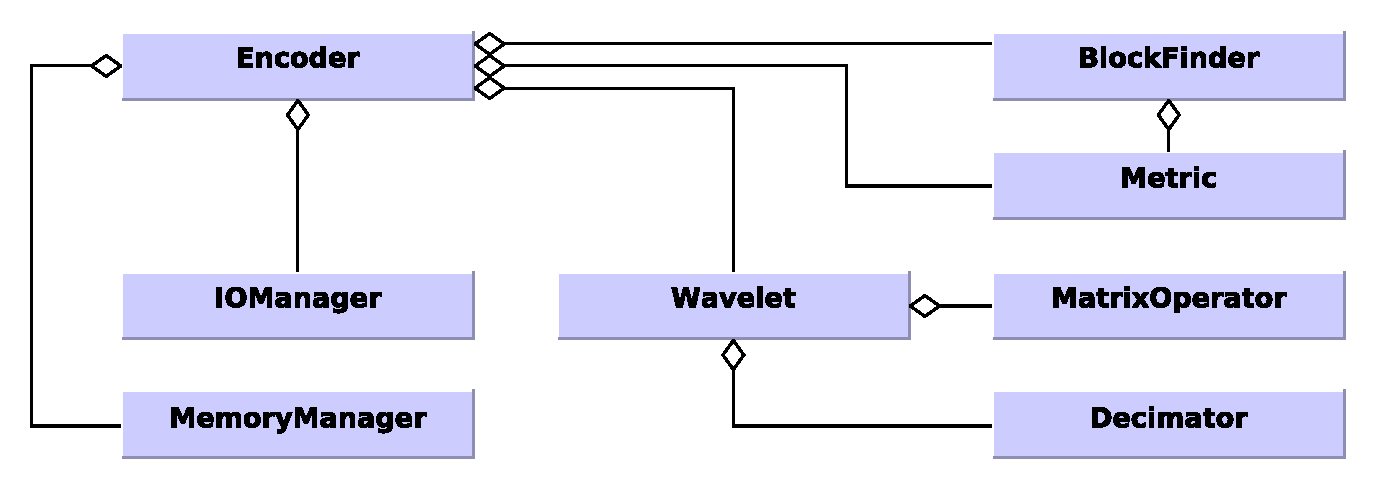
\includegraphics[scale=0.6]{inc/graphics/modules.pdf}
  \caption{Cхема модулей разрабатываемой системы}
  \label{fig:modules}
\end{figure}

Модуль \texttt{Encoder} является основным модулем разрабатываемой системы, в котором происходит весь процесс обработки 
графических данных от чтения графических данных из файла до записи закодированных графических данных в файл.
Содержит функции:

\begin{itemize}
 \item функция кодирования исходных графических данных,
 \item функция декодирования преобразованных графических данных.
\end{itemize}

Модуль \texttt{BlockFinder} вычисляет блоки, к которым будет применено вейвлетное преобразование. Содержит функцию
поиска блоков, принимающую на вход графические данные и возвращающую вычисленные блоки.

Модуль \texttt{IOManager} чтения/записи данных в файл при чтении получает от управляющего модуля имя файла и возвращает прочитанные графические данные, 
при записи получает от управляющего модуля имя файла и графические данные и возвращает результат выполнения операции записи. 
Содержит следующие функции:
\begin{itemize}
 \item функция чтения графических данных из файла,
 \item функция записи преобразованных графических данных в файл,
 \item функция чтения преобразованных графических данных из файла.
\end{itemize}

Модуль \texttt{MemoryManager} управляет памятью, необходимой для выполнения расчетов во время применения вейвлетного преобразования.
Содержит следующие функции:
\begin{itemize}
 \item функция выделения блока памяти для расчетов,
 \item функция освобождения выделенной памяти,
 \item функция копирования графических данных во временную память для применения прямого вейвлетного преобразования,
 \item функция копирования преобразованых данных во временную память для применения обратного вейвлетного преобразования.
\end{itemize}

Модуль вейвлетных преобразований \texttt{Wavelet} получает на вход графические данные и параметры преобразования, 
применяет к данным указанное преобразование, возвращает преобразованные данные. Содержит следующие функции:
\begin{itemize}
\item функция выполнения прямого вейвлетного преобразования,
\item функция выполнения обратного вейвлетного преобразования.
\end{itemize}

Для работы модуля вейвлетных преобразований требуется вспомогательный модуль работы с матрицами \texttt{MatrixOperator}, 
который производит умножение матрицы на вектор, а так же составление матриц для указанного вейвлетного преобразования. Содержит следующие функции:
\begin{itemize}
\item функция составления матрицы преобразования указанной размерности для указанной системы коэффициентов,
\item функция получения набора коэффициентов указанной системы коэффициентов,
\item функция умножения матрицы на вектор графических данных,
\item функция транспонирования матрицы.
\end{itemize}
Алгоритм составления матрицы представлен на рисунке 

Модуль выбора значимых коэффициентов \texttt{MatrixOperator} получает от модуля \texttt{Wavelet} графические данные и степень сжатия, 
удаляет указанную часть данных, возвращает обработанные данные. Содержит следующие функции: 
\begin{itemize}
\item функция удаления части графических данных,
\item функция поиска порядковой статистики.
\end{itemize}

\chapter{Технологический раздел}
\label{cha:impl}

В данном разделе описано изготовление и требование всячины. Кстати,
в Latex нужно эскейпить подчёркивание (писать <<\verb|some\_function|>> для \Code{some\_function}).

Для вставки кода есть пакет \Code{listings}. К сожалению, пакет \Code{listings} всё ещё
работает криво при появлении в листинге русских букв и кодировке исходников utf-8.
В данном примере он (увы) на лету конвертируется в koi-8 в ходе сборки pdf.

Есть альтернатива \Code{listingsutf8}, однако она работает лишь с
\Code{\textbackslash{}lstinputlisting}, но не с окружением \Code{\textbackslash{}lstlisting}

Вот так можно вставлять псевдокод (питоноподобный язык определен в \Code{listings.inc.tex}):

\begin{lstlisting}[style=pseudocode,caption={Алгоритм оценки дипломных работ}]
def EvaluateDiplomas():
    for each student in Masters:
        student.Mark := 5
    for each student in Engineers:
        if Good(student):
            student.Mark := 5
        else:
            student.Mark := 4
\end{lstlisting}

Еще в шаблоне определен псевдоязык для BNF:

\begin{lstlisting}[style=grammar,basicstyle=\small,caption={Грамматика}]
  ifstmt -> "if" "(" expression ")" stmt |
            "if" "(" expression ")" stmt1 "else" stmt2
  number -> digit digit*
\end{lstlisting}

В листинге~\ref{lst:sample01} работают русские буквы. Сильная магия. Однако, работает
только во включаемых файлах, прямо в \TeX{} нельзя.

% Обратите внимание, что включается не ../src/..., а inc/src/...
% В Makefile есть соответствующее правило для inc/src/*,
% которое копирует исходные файлы из ../src и конвертирует из UTF-8 в KOI8-R.
% Кстати, поэтому использовать можно только русские буквы и ASCII,
% весь остальной UTF-8 вроде CJK и египетских иероглифов -- нельзя.

\lstinputlisting[language=C,caption=Пример (\Code{test.c}),label=lst:sample01]{inc/src/test.c}

% Для вставки реального кода лучше использовать \texttt{\textbackslash lstinputlisting} (который понимает
% UTF8) и стили \Code{realcode} либо \Code{simplecode} (в зависимости от размера куска).




Можно также использовать окружение \Code{verbatim}, если \Code{listings} чем-то не
устраивает. Только следует помнить, что табы в нём <<съедаются>>. Существует так же команда \Code{\textbackslash{}verbatiminput} для вставки файла.

\begin{verbatim}
a_b = a + b; // русский комментарий
if (a_b > 0)
    a_b = 0;
\end{verbatim}

%%% Local Variables:
%%% mode: latex
%%% TeX-master: "rpz"
%%% End:

\chapter{Экспериментальный раздел}
\label{cha:research}

В данном разделе проводятся вычислительные эксперименты.
А на рис.~\ref{fig:spire01} показана схема мыслительного процесса автора...

\begin{figure}
  \centering
  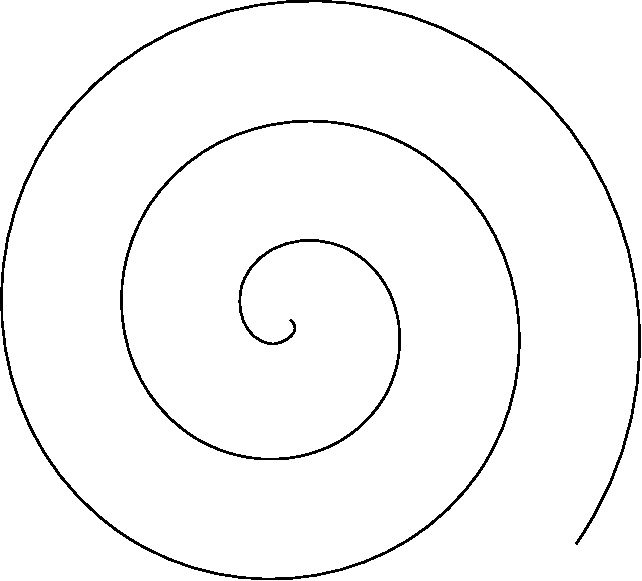
\includegraphics[width=\textwidth]{inc/svg/pic01}
  \caption{Как страшно жить}
  \label{fig:spire01}
\end{figure}


%%% Local Variables:
%%% mode: latex
%%% TeX-master: "rpz"
%%% End:


\backmatter %% Здесь заканчивается нумерованная часть документа и начинаются ссылки и
            %% заключение

\chapter{Заключение}

В рамках курсового проекта были достигнуты следующие цели:
\begin{itemize}
\item описан конечный автомат состояний протокола на основе его спецификации и с учётом отслеживания таймаутов;
\item cпроектировано взаимодействия подсистем;
\item спроектированы алгоритмы обработки соединений в одном потоке выполнения и их распределеление между потоками;
\item написан исходный код программы;
\item создан сценарий сборки системы, создана записка, проведены тесты;
\item созданы системы системного тестирования.
\end{itemize}

Основным результатом работы является реализация SMTP-сервера, обеспечивающего локальную доставку и добавление в очередь удаленной доставки.


% % Список литературы при помощи BibTeX
% Юзать так:
%
% pdflatex rpz
% bibtex rpz
% pdflatex rpz

\bibliographystyle{gost780u}
\bibliography{rpz}

%%% Local Variables: 
%%% mode: latex
%%% TeX-master: "rpz"
%%% End: 


\appendix   % Тут идут приложения

\chapter{Системы коэффициентов Добеши}
\label{cha:koef}

%  \begin{table}
%  \caption{Ортогональные нормированные коэффициенты Добеши низких порядков}
% \begin{tabular}{|p{1cm}|p{1cm}|p{1cm}|p{1cm}|p{1cm}|p{1cm}|p{1cm}|p{1cm}|p{1cm}|}
% \hline
%   D2  & D4 & D6 & D8 & D10 & D12 & D14 & D16 & D18 & D20 \\
%   \hline
%   1 & 0.6830127 & 0.47046721   &   0.32580343    &  0.22641898   &   0.15774243   &   0.11009943   &   0.07695562   &0.05385035&0.03771716 \\
%   \hline
% \end{tabular}
%  \end{table}
\begin{table}[ht]\tiny
\caption{Ортогональные нормированные коэффициенты Добеши низких порядков}
\rotatebox{90}{
  \begin{tabular}{|p{0.3cm}|p{1.4cm}|p{1.4cm}|p{1.4cm}|p{1.2cm}|p{1.5cm}|p{1.5cm}|p{1.2cm}|p{1.2cm}|p{2cm}|}
  \hline
  D2 & D4 & D6 & D8 & D10 & D12 & D14 & D16 & D18 & D20 \\
  \hline
  1 & 0.6830127&0.47046721&0.32580343&0.22641898&0.15774243&0.11009943&0.07695562&0.05385035&0.03771716\\
  \hline
  1&1.1830127&1.14111692&1.01094572&0.85394354&0.69950381&0.56079128&0.44246725&0.34483430&0.26612218\\
  \hline
&0.3169873&0.650365&0.8922014&1.02432694&1.06226376&1.03114849&0.95548615&0.85534906&0.74557507\\
\hline
&-0.1830127&-0.19093442&-0.03957503&0.19576696&0.44583132&0.66437248&0.82781653&0.92954571&0.97362811\\
\hline 
&&-0.12083221&-0.26450717&-0.34265671&-0.31998660&-0.20351382&-0.02238574&0.18836955&0.39763774\\
\hline 
&&0.0498175&0.0436163&-0.04560113&-0.18351806&-0.31683501&-0.40165863&-0.41475176&-0.35333620\\
\hline 
&&&0.0465036&0.10970265&0.13788809&0.1008467&6.68194092e-4&-0.13695355&-0.27710988\\
\hline 
&&&-0.01498699&-0.00882680&0.03892321&0.11400345&0.18207636&0.21006834&0.18012745\\
\hline 
&&&&-0.01779187&-0.04466375&-0.05378245&-0.02456390&0.043452675&0.13160299\\
\hline 
&&&&4.71742793e-3&7.83251152e-4&-0.02343994&-0.06235021&-0.09564726&-0.10096657\\
\hline 
&&&&&6.75606236e-3&0.01774979&0.01977216&3.54892813e-4&-0.04165925\\
\hline 
&&&&&-1.52353381e-3&6.07514995e-4&0.01236884&0.03162417&0.04696981\\
\hline 
&&&&&&-2.54790472e-3&-6.88771926e-3&-6.67962023e-3&5.10043697e-3\\
\hline 
&&&&&&5.00226853e-4&-5.54004549e-4&-6.05496058e-3&-0.01517900\\
\hline 
&&&&&&&9.55229711e-4&2.61296728e-3&1.97332536e-3\\
\hline 
&&&&&&&-1.66137261e-4&3.25814671e-4&2.81768659e-3\\
\hline 
&&&&&&&&-3.56329759e-4&-9.69947840e-4\\
\hline 
&&&&&&&&5.5645514e-5&-1.64709006e-4\\
\hline 
&&&&&&&&&1.32354367e-4\\
\hline 
&&&&&&&&&-1.875841e-5\\
\hline 
  \end{tabular}
%   \label{tab:t2}
}
\end{table}
\chapter{Еще картинки}
\label{cha:appendix2}

\begin{figure}
\centering
\caption{Еще одна картинка, ничем не лучше предыдущей. Но надо же как-то заполнить место.}
\end{figure}

%%% Local Variables: 
%%% mode: latex
%%% TeX-master: "rpz"
%%% End: 


\end{document}

%%% Local Variables:
%%% mode: latex
%%% TeX-master: t
%%% End:
